\appendix
%\renewcommand*{\thesection}{\arabic{section}}
\renewcommand*{\thesubsection}{\thesection.\arabic{subsection}}
\renewcommand*{\thesubsubsection}{\thesubsection.\arabic{subsubsection}}

\section{WBS Tables}
\label{sec:wbs}
% 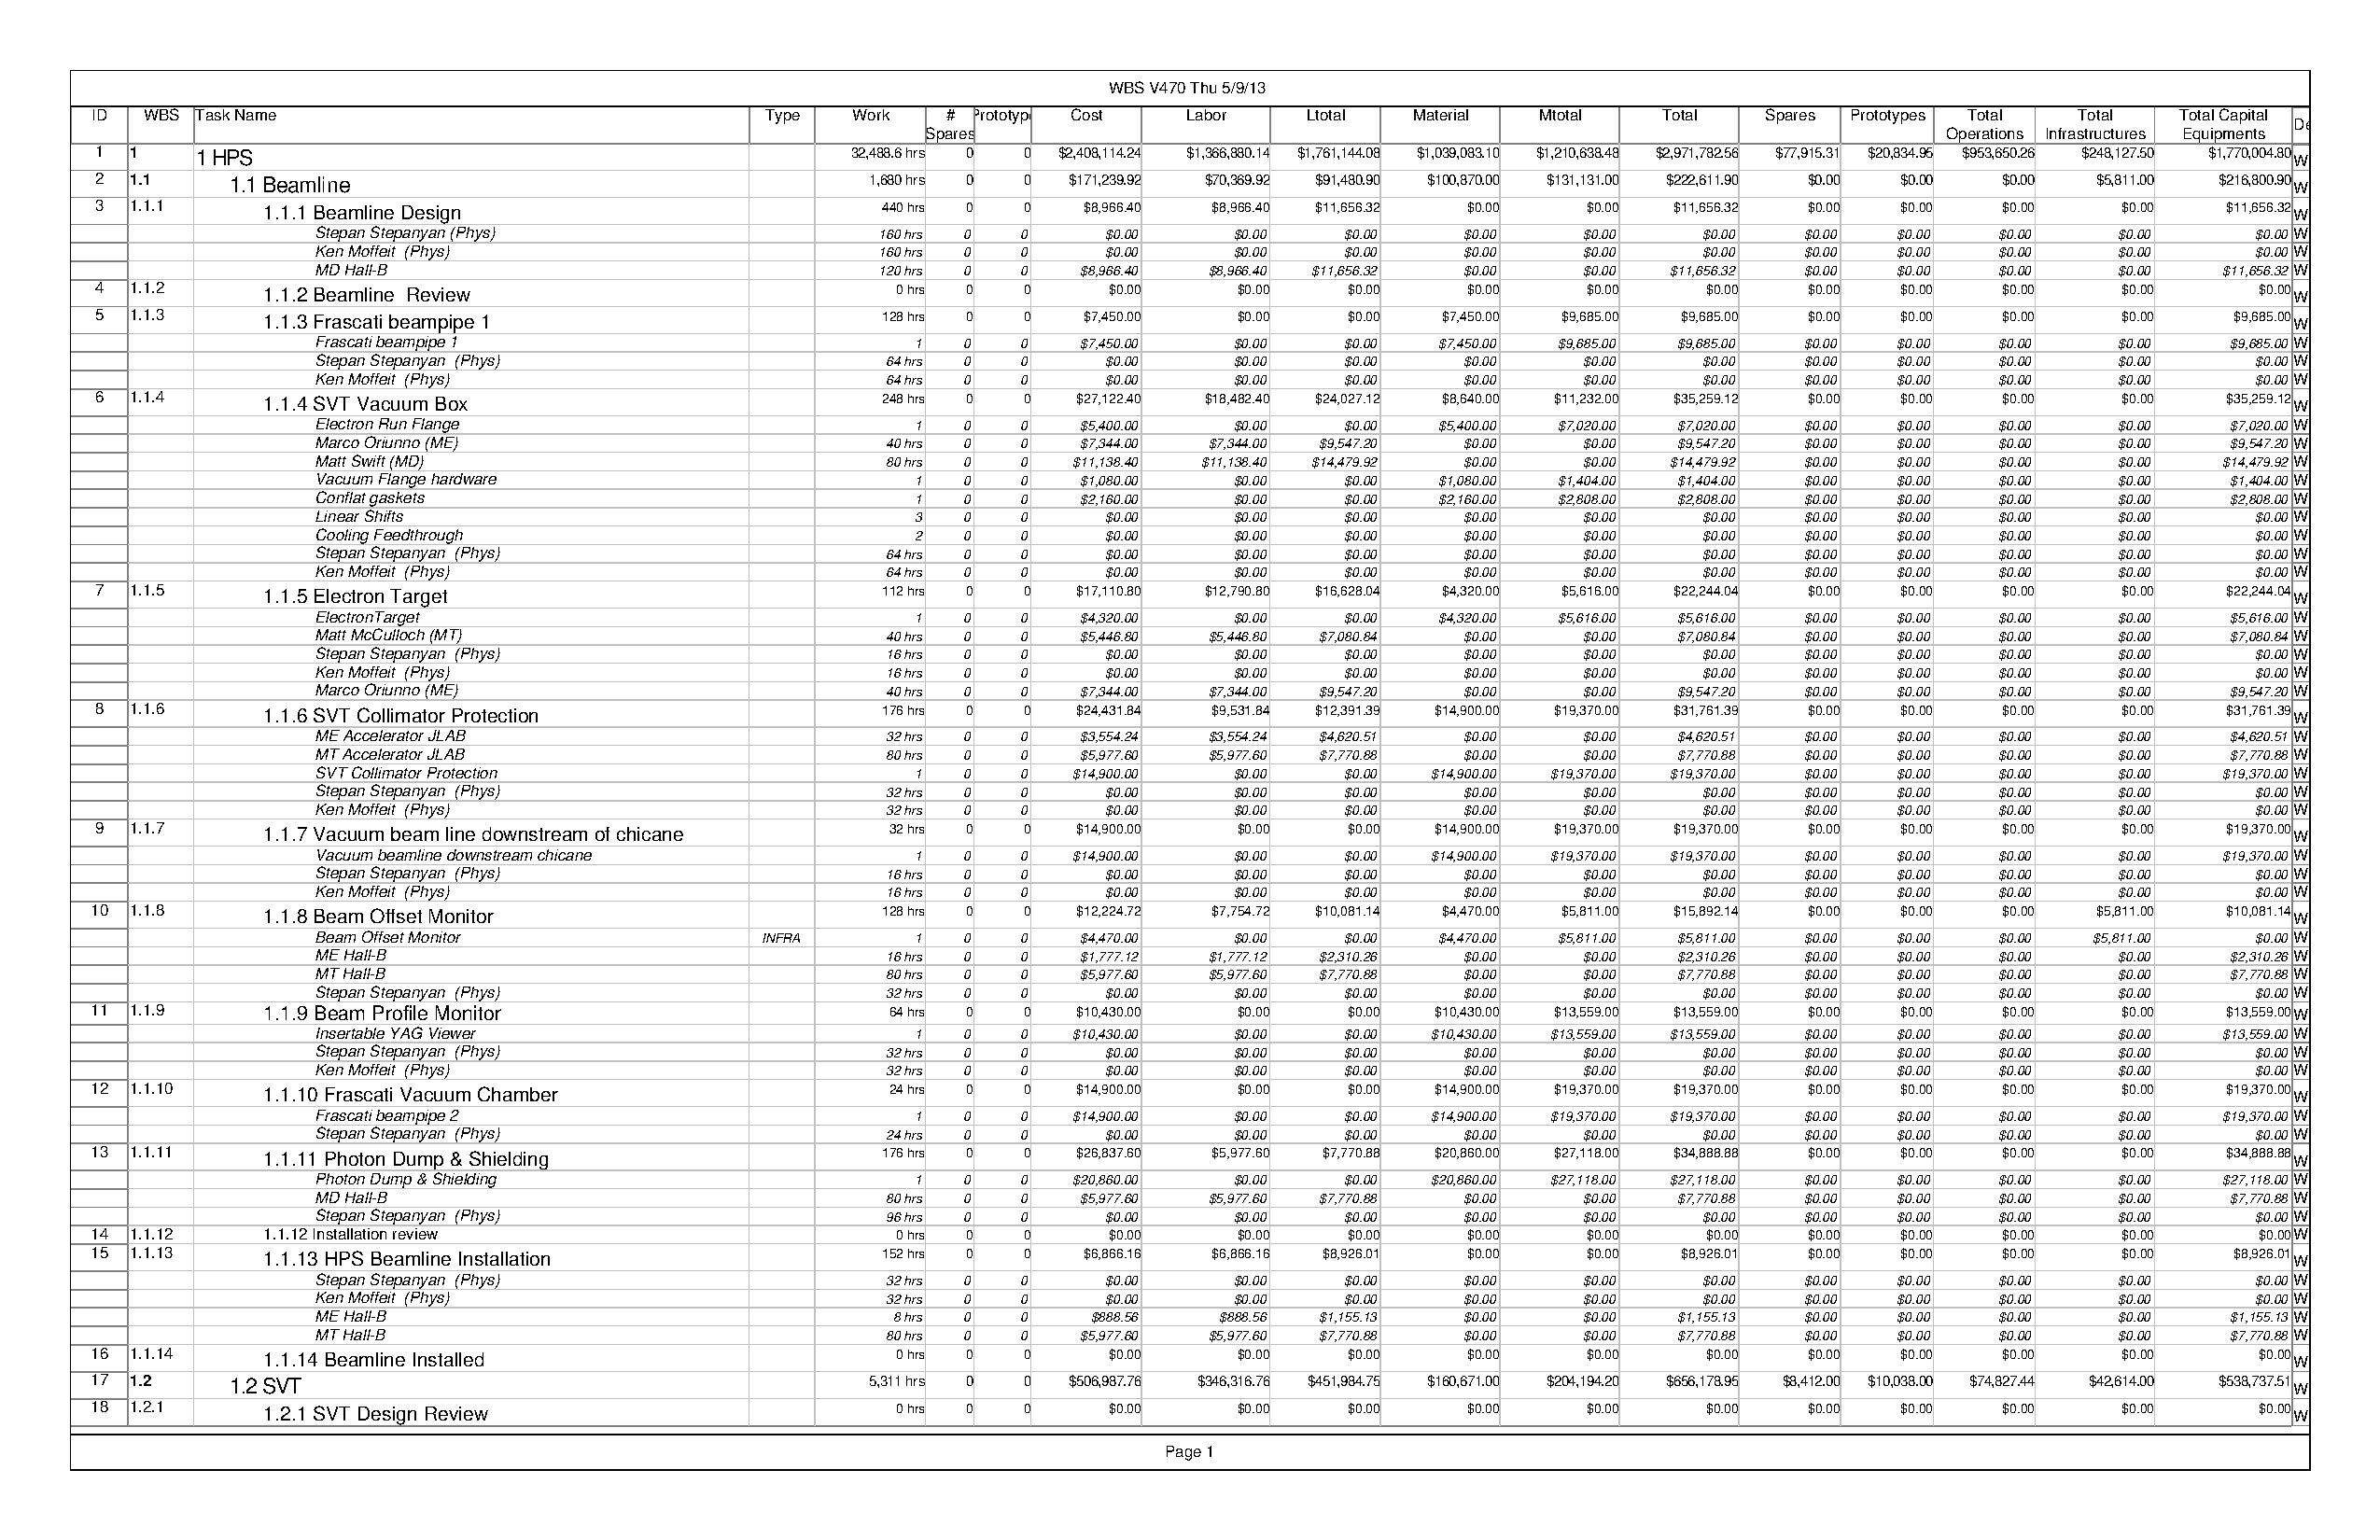
\includepdf[pages=1-9,angle=90,scale=0.8,offset=0 -0.5in]{cost_schedule/HPSV470.pdf}
\begin{center}
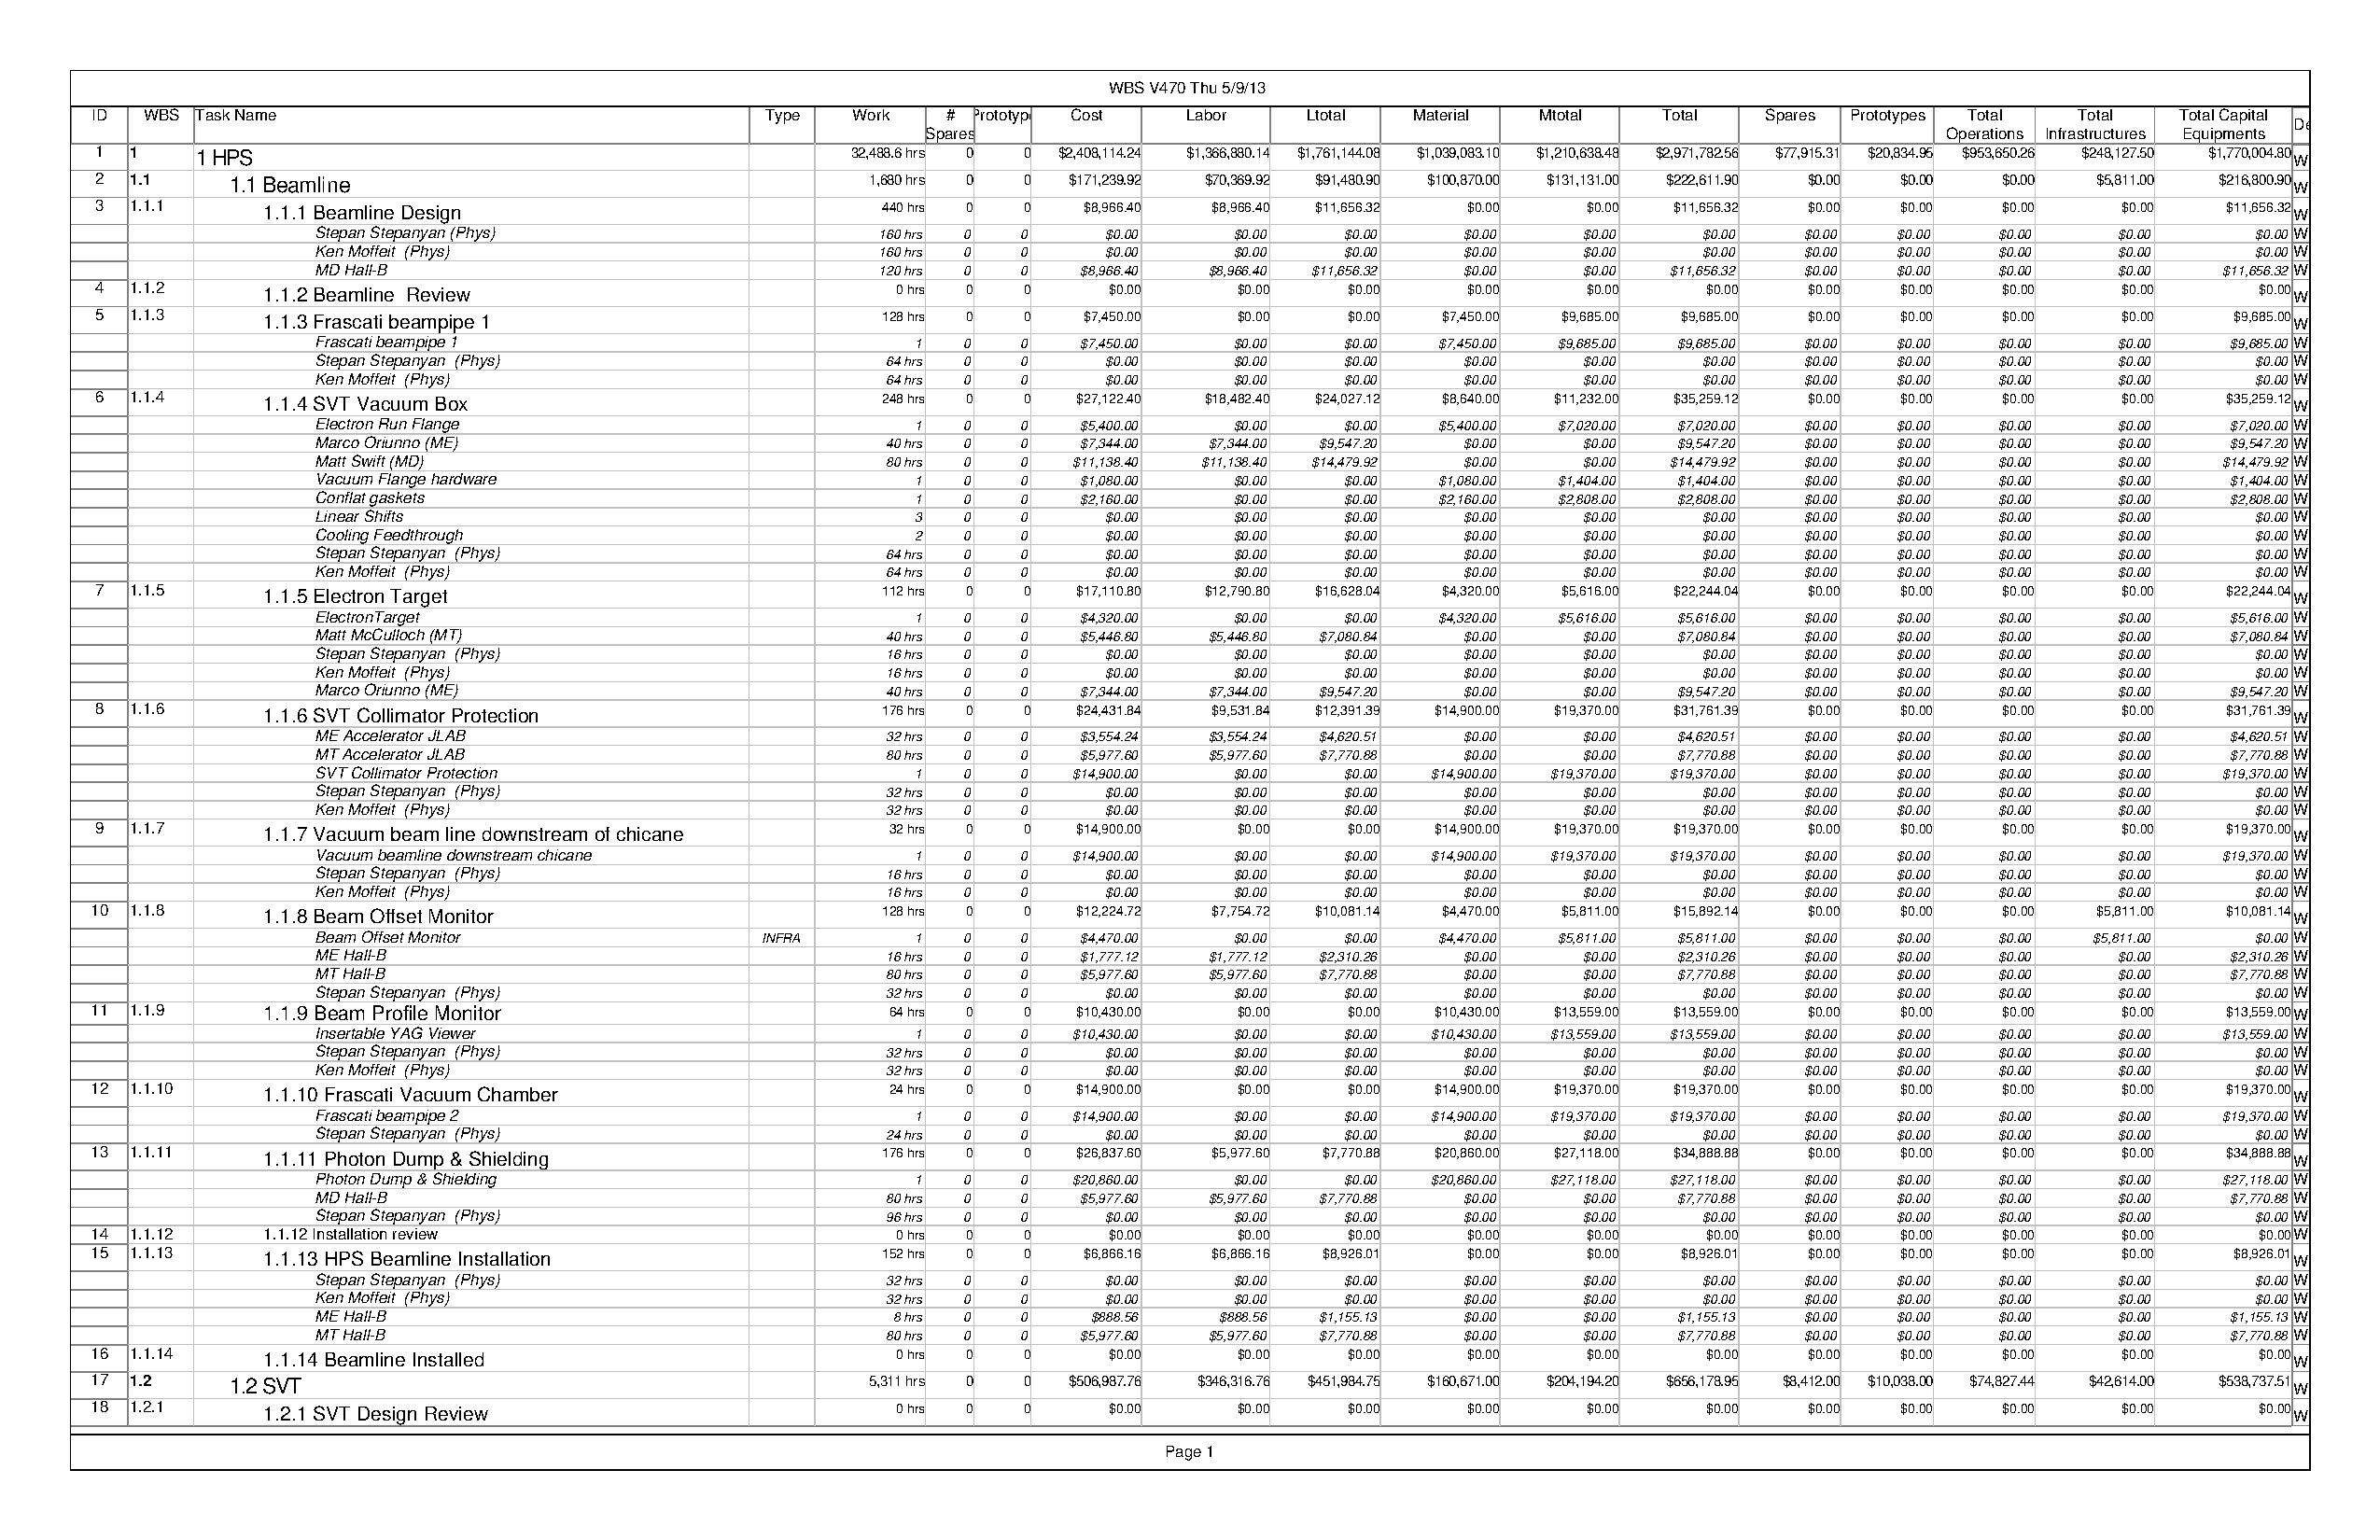
\includegraphics[page=1,angle=90,height=0.9\textheight]{cost_schedule/HPSV470.pdf} 
\end{center}

\begin{center}
\includegraphics[page=2,angle=90,height=\textheight]{cost_schedule/HPSV470.pdf} 
\end{center}

\begin{center}
\includegraphics[page=3,angle=90,height=\textheight]{cost_schedule/HPSV470.pdf} 
\end{center}

\begin{center}
\includegraphics[page=4,angle=90,height=\textheight]{cost_schedule/HPSV470.pdf} 
\end{center}

\begin{center}
\includegraphics[page=5,angle=90,height=\textheight]{cost_schedule/HPSV470.pdf} 
\end{center}

\begin{center}
\includegraphics[page=6,angle=90,height=\textheight]{cost_schedule/HPSV470.pdf} 
\end{center}

\begin{center}
\includegraphics[page=7,angle=90,height=\textheight]{cost_schedule/HPSV470.pdf} 
\end{center}

\begin{center}
\includegraphics[page=8,angle=90,height=\textheight]{cost_schedule/HPSV470.pdf} 
\end{center}

\begin{center}
\includegraphics[page=9,angle=90,height=\textheight]{cost_schedule/HPSV470.pdf} 
\end{center}

%WBS tables:

%\clearpage
%\begin{figure*}[ht]
%\centering
%\vspace*{-5mm}
%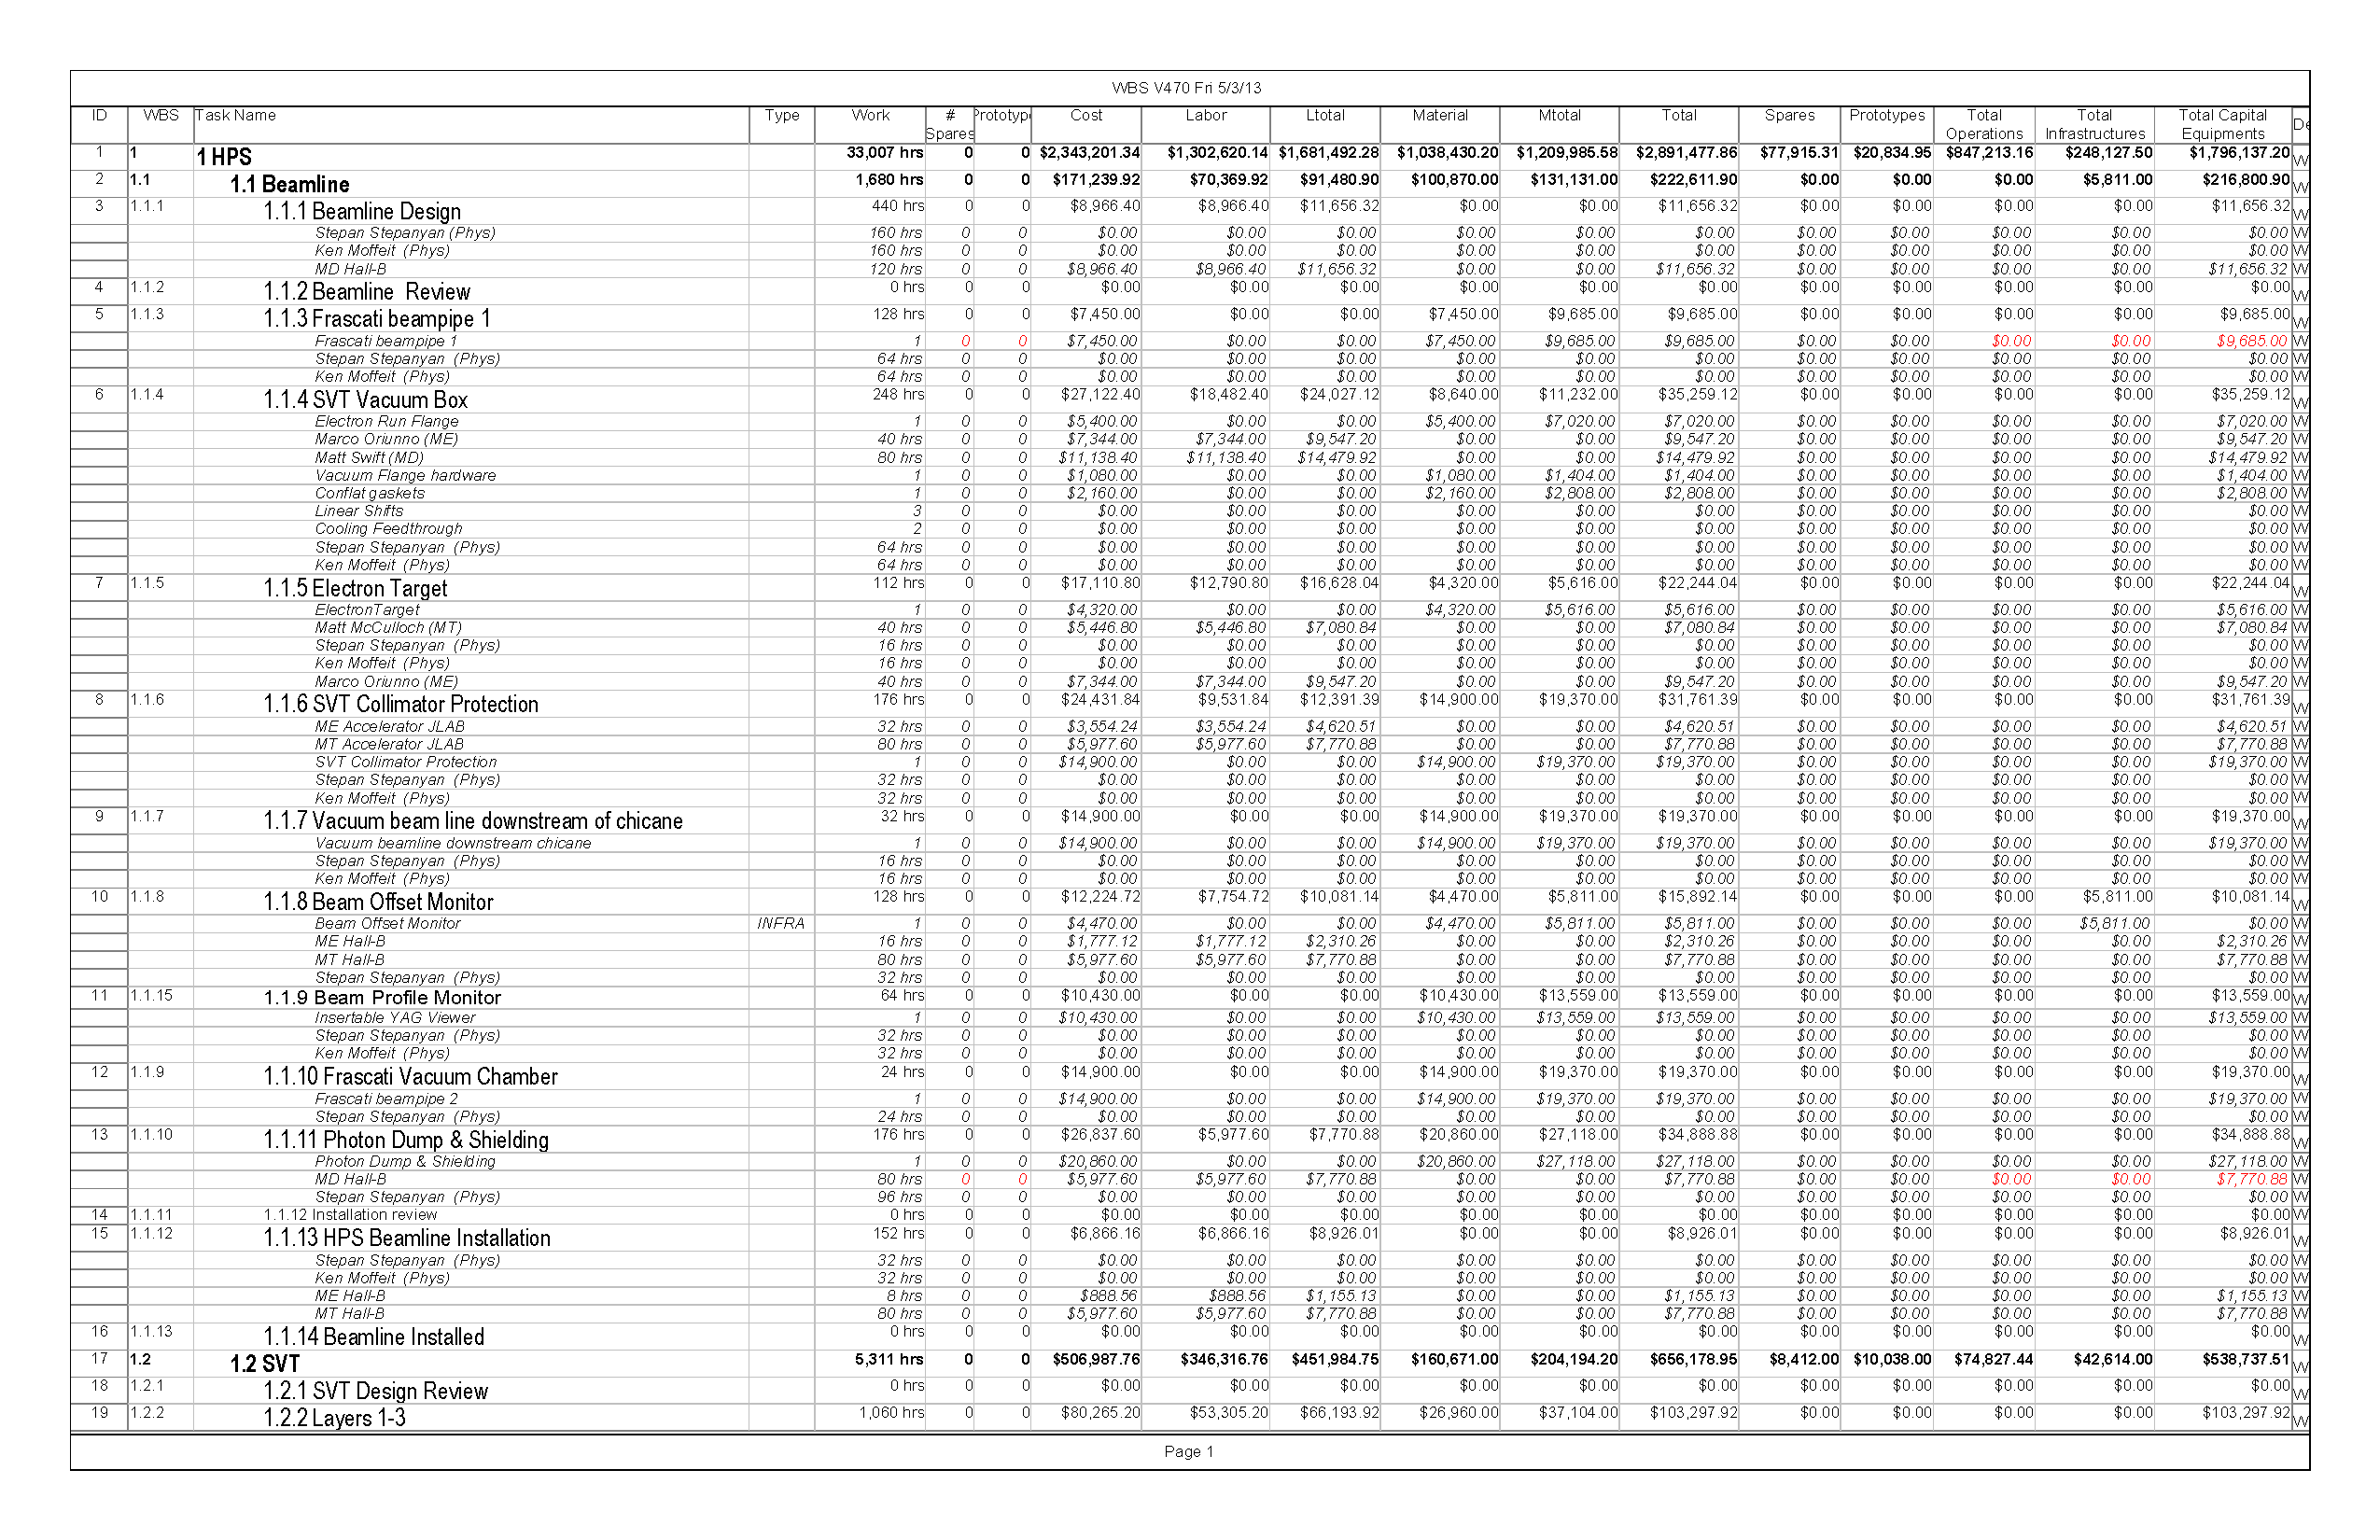
\includegraphics[angle=0,width=\textwidth]{cost_schedule/HPSV470p1} 
%\caption{HPS WBS.}
%\label{fig:schedulea}
%\end{figure*}

%\begin{rotate}{90}

\section{Additions and improvements to the HPS setup using non-DOE sources of funding}

While the proposed baseline equipment will be sufficient to carry out the proposed measurements, the HPS collaboration is 
seeking funding from non-DOE sources to improve and enhance capabilities of the HPS detector. Plans for improvements 
include a light monitoring system, new preamplifiers, and large area APDs for the ECal. The HPS collaborators from IPN Orsay have applied for 
a number of European grants, including European Research Council (ERC) Advanced Grant 2013 to purchase APDs, for 
manpower costs to replace the old ones, to design and build 
new preamplifier boards, and to assemble and test the ECal with the new modules. The total cost of replacing all ECal APDs is about $500$K\$. 
These grants also include the light monitoring system. If successful, European funding will cover most of the ECal modifications, 
and will significantly reduce the support needed from DOE for the more modest upgrades we have proposed above. 

Besides ECal improvements, the collaboration intends to add a muon detector to the HPS setup. Collaborators from the College 
of William\&Mary (PI Prof. Keith Griffioen) together with collaborators from Rutgers University (PI Prof. Yuri Gerstein) 
and Old Dominion University (PI Prof. Lary Weinstein) submitted an MRI proposal to NSF for the Muon System, requesting $\sim 300$k.  

The details of ECal improvements, and the motivation and description of the muon system are presented below. 

\subsection{Improvements to ECal}

\begin{enumerate}
\item {\bf Light monitoring system}

For an experiment like HPS, where backgrounds must be well understood and need to be strongly suppressed, the trigger bias must be minimized. In particular, having stable, known, and uniform thresholds at the trigger readout is necessary in order to avoid  bias in the 
event selection. Such uniformity and stability can be achieved with the installation of an online gain monitoring 
system. This system will introduce short light pulses into the front face of the crystals. The crystals already have fiber holders attached, allowing implementation of this system without having to modify the crystals or wrapping. 

Optical fibers will be used to transmit light from a calibration  source to the crystals to test the response of the APDs. The response of the system could change in time because of 
losses in crystal transparency due to radiation damage or because of gain variations of the APDs. 
Such a calibration system has been developed for several experiments (CMS at CERN for instance) with various light sources. The system for the ECal 
will be developed at IPN Orsay during 2013 and in the first half of 2014, and will be ready for installation at JLAB for the commissioning run in the fall of 2014. Each module will have a red and blue mono-color LED light source for monitoring purposes. 
Blue light transmission, corresponding to the domain of the crystal's emission spectrum, is very sensitive to the presence of color centers which are produced by radiation damage. So the blue light source will monitor variations of the response in the main domain of the spectrum.
 %Impurities can anneal at room temperature and such monitoring can be sensitive to increasing of output as well, when the radiation exposure is reduced for a long period of time. 
The response to red light is less sensitive to the color centers,  and so permits monitoring the APD gains more directly. Thus the use of two colors separates gain variations due to the 
APD and electronics from those due to changes in the crystal transparency, and provides clear information on the state of the electronics. 
The main challenge for the system is to guarantee stability at a level of $2\%$. The test of the system will be carried-out at
IPN Orsay, in order to study its efficacy and also to test the radiation resistance of the various materials.

\item {\bf Modifications to the side brackets to accommodate fiber bundles for the light monitoring system} -
A light monitoring system was not used during the test run. While the design of the ECal enclosure was done in such a way that it can 
accommodate optical fibers attached to the front face of crystals, the side plates that hold the crystal frames do not have inlets for the accompanying fiber bundles.
Space is available on the side plates for a straight-forward modification which will allow the addition of a light monitoring system.  
    
\item {\bf New low-voltage power supply} - The existing low voltage power supply is a manually controlled, single output power supply 
that feeds the four ECal motherboards through a custom-made patch panel. The present system cannot control the voltage supplied to preamplifiers at different
parts of the ECal, and controlling or resetting them remotely has proved to be very inconvenient, requiring frequent access to the Hall, especially during commissioning. Newly available low voltage power supplies are much more flexible. The one that is the most suitable for the
ECal APD preamplifiers is the WIENER MPV 8008LD. This power supply is being used at JLAB and the control software exists, so it will be easy to incorporate it into HPS.     

\item {\bf New preamplifiers} - A low noise, low gain preamplifiers will be needed to take advantage of increased signal on the input of FADC after removing the spliter. The impact of the lower noise/threshold system is twofold: first it 
will improve the ECal's energy resolution; and second it will make the ECal sensitive to minimum ionizing particles which pass through the crystals transversely. With sensitivity to cosmic ray muons, which will pass through the ECal transversely when it is installed in HPS, the Ecal crystals can be calibrated for MIPS, and their effective gains balanced.  HPS collaborators from INFN Genova have shown that with such a low noise, low threshold system, the ECal can distinguish the MIP energy deposition from noise, see left plot on Figure \ref{fig:mip10x10}.

%\begin{figure*}[t]
%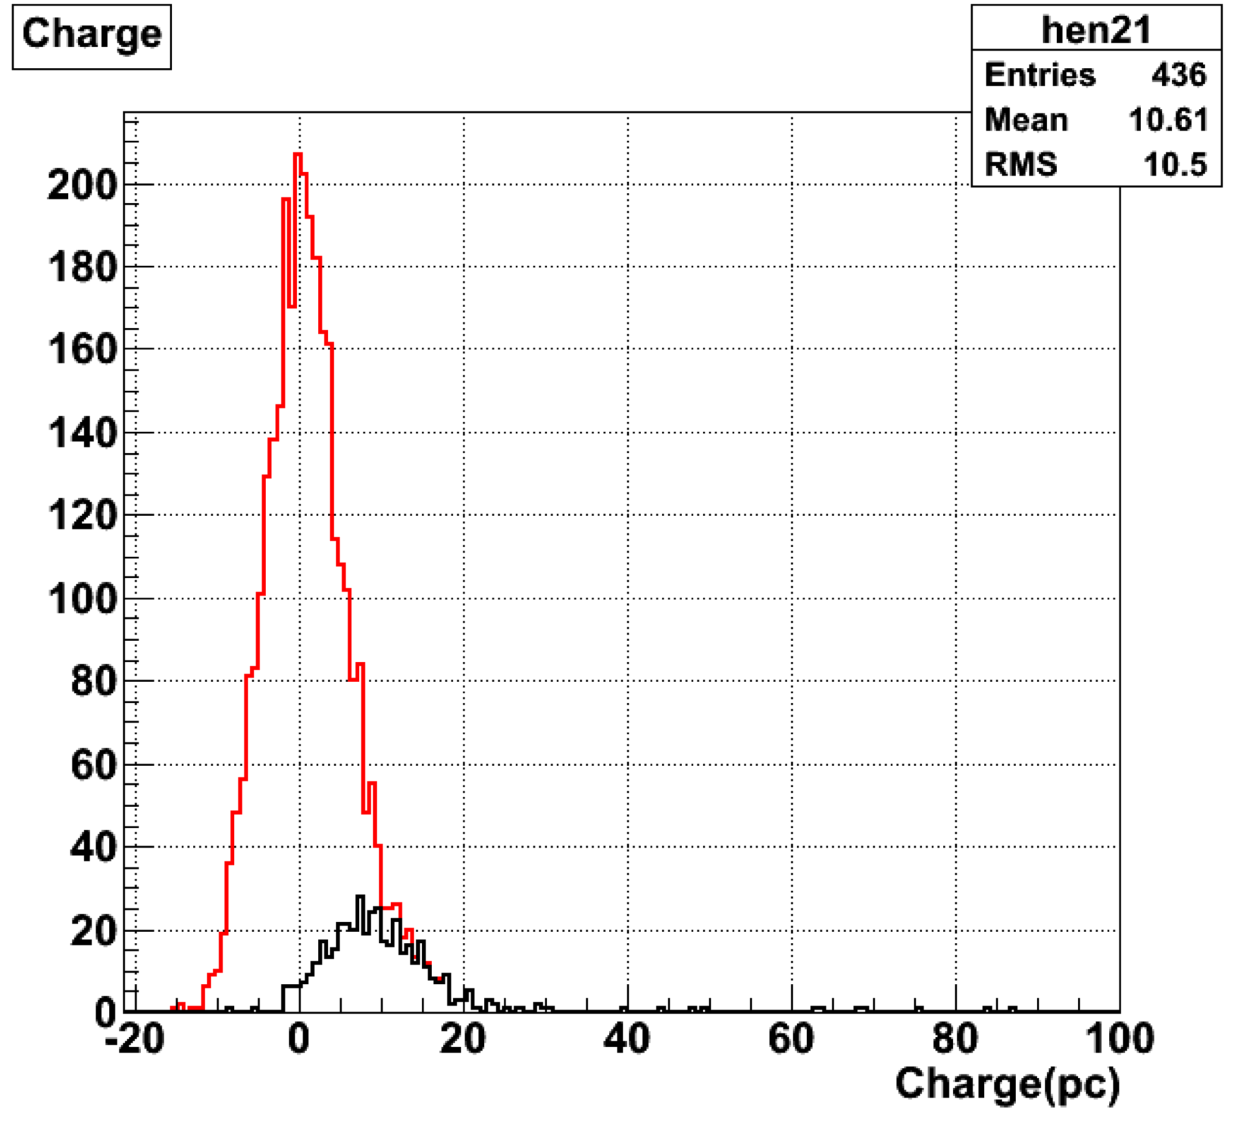
\includegraphics[scale=0.4]{ecal/MIP_5x5_APD.png}
%\caption{\small{Charge distribution from readout of the HPS calorimeter crystal with Hamamatsu S8664-55 APD, and the new low noise amplifier board. The red line histogram corresponds to the charge distribution for all triggers coming from the scintillators positioned above and below the crystal. The black line shows the distribution for hits in the crystal within $100$ ns of the trigger signal. }}\label{fig:mip5x5}
%\end{figure*}


\item{\bf Possibilities with new APDs} - Installing new APDs on the existing crystals will significantly improve the ECal performance, but doing so is expensive,  so replacement is only being considered if a funding source beyond DOE HEP is secured. Replacing the old $5\times 5$ mm$^2$ 
Hamamatsu S8664-55 APDs with $10\times 10$ mm$^2$, Hamamatsu S8664-1010 will improve two critical characteristics of the present calorimeter modules. First, the new APDs from Hamamatsu have much better performance than the ones which are currently installed. Data from Hamamatsu shows that APDs made from the same wafer have excellent gain uniformity. With $\pm 10\%$ known uniformity 
at the gain of $100$, the required variations in bias voltage are only $\sim 4.5$ V. Even for large samples of APDs (~1300),  the required bias voltage differences are ~50 V, which is half that of the current APDS. The ECal supplies bias voltage to groups of APDs, so with new APDs, with their smaller voltage-gain variations, it will be possible to achieve much better 
uniformity in the response of the calorimeter modules, and consequently better uniformity in trigger thresholds. 

Secondly, the new APDs have a $4$ times larger readout area, ensuring $4$ times more light collection and therefore $4$ times larger signals. This will allow the use of lower gain amplifier modules which in turn will decrease electronic noise. Tests 
performed for another calorimeter, now in production at INFN Genova for JLAB Hall-B, showed that amplifier boards 
with a factor 2 lower gains have a noise level $<5$ MeV. The energy deposition in the HPS PbWO$_4$ crystals  
from minimum ionizing cosmic muons passing transversely to the crystal axis is $\sim 15$ MeV. Moving the energy thresholds 
close to $5$ MeV will allow the MIP peak to be clearly distinguished, and will let the calorimeter  be calibrated and monitored with cosmic muons. The HPS collaborators 
from the INFN group have performed the first tests of the Hamamtsu $10\times 10$ mm$^2$ APDs and a new amplifier board on HPS crystals. In 
Figure \ref{fig:mip10x10}, the charge distribution of a single crystal system is shown for $5\times 5$ mm$^2$ (left) and $10\times 
10$ mm$^2$ (right) APDs. A coincidence signal from scintillator telescopes positioned above and below the module provides the trigger. 
The crystal was positioned horizontally as it would be in HPS, so the cosmic muons would pass through it perpendicular to the crystal axis. The red line 
histogram is for all events triggered by the scintillation telescope and corresponds to the noise. The black line histogram corresponds 
to the charge detected within $100$ ns of the trigger time. The MIP peak is clearly visible and well isolated from the noise 
for the S8664-1010 APD readout. For  the S8664-55 APD, the MIP signal is also seen, but its charge distribution is under the noise peak and it
does not have well defined peak position. Using MIP calibration in conjunction with the light monitoring system will ensure stable and reliable performance of the ECal and the trigger system. As a bonus, the lower noise will allow the use of lower  thresholds and improve the calorimeter's energy resolution. The new amplifier boards have to be designed to work with new APDs. 

\begin{figure*}[t]
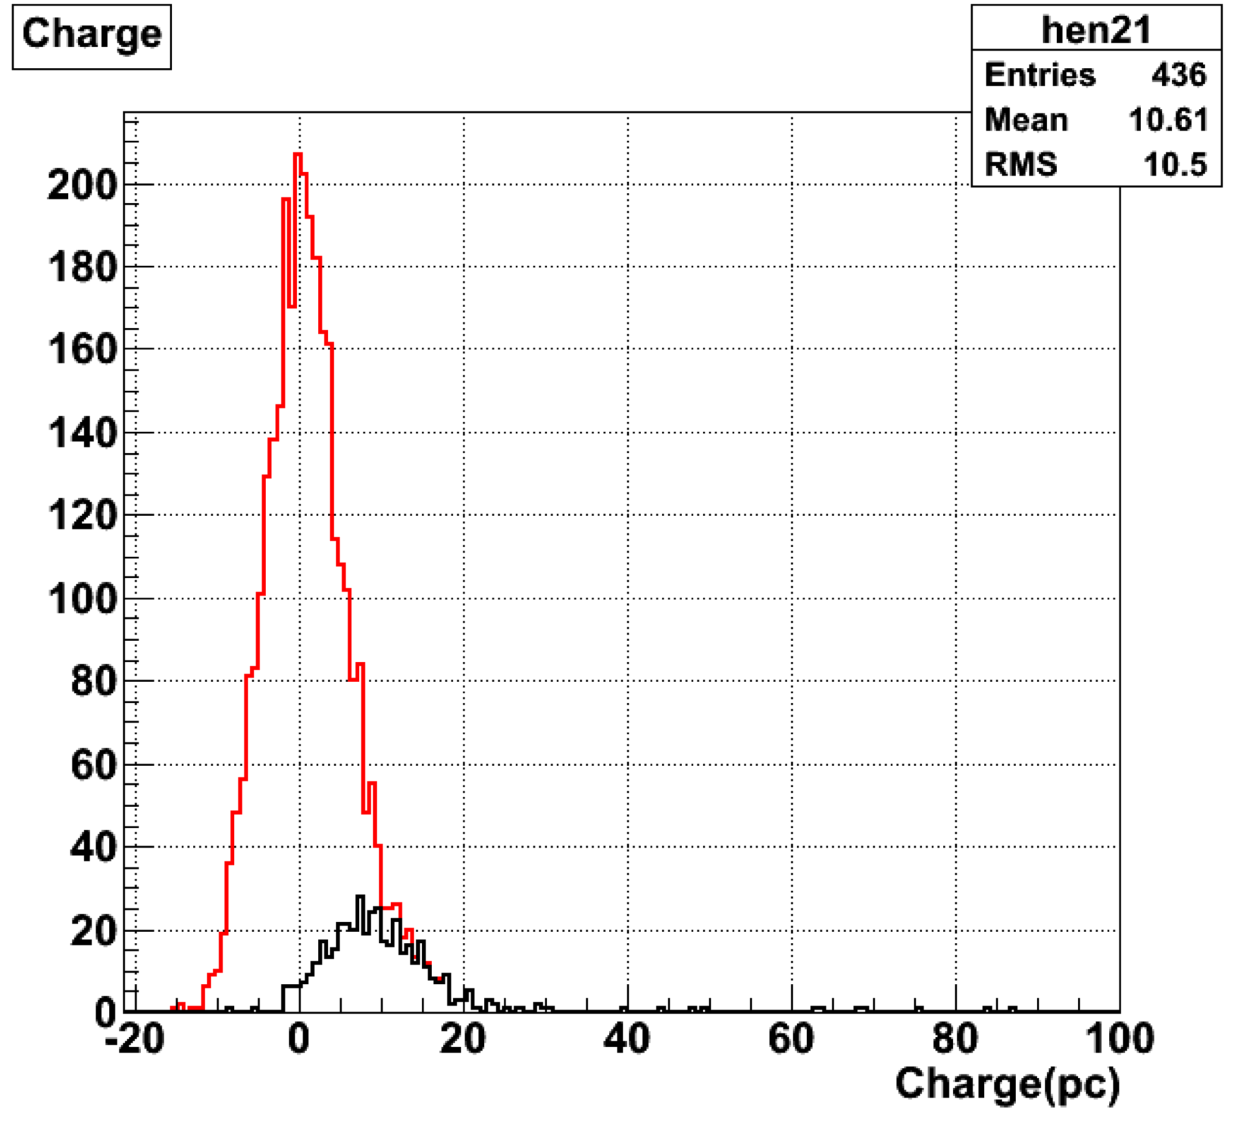
\includegraphics[scale=0.37]{ecal/MIP_5x5_APD.png}
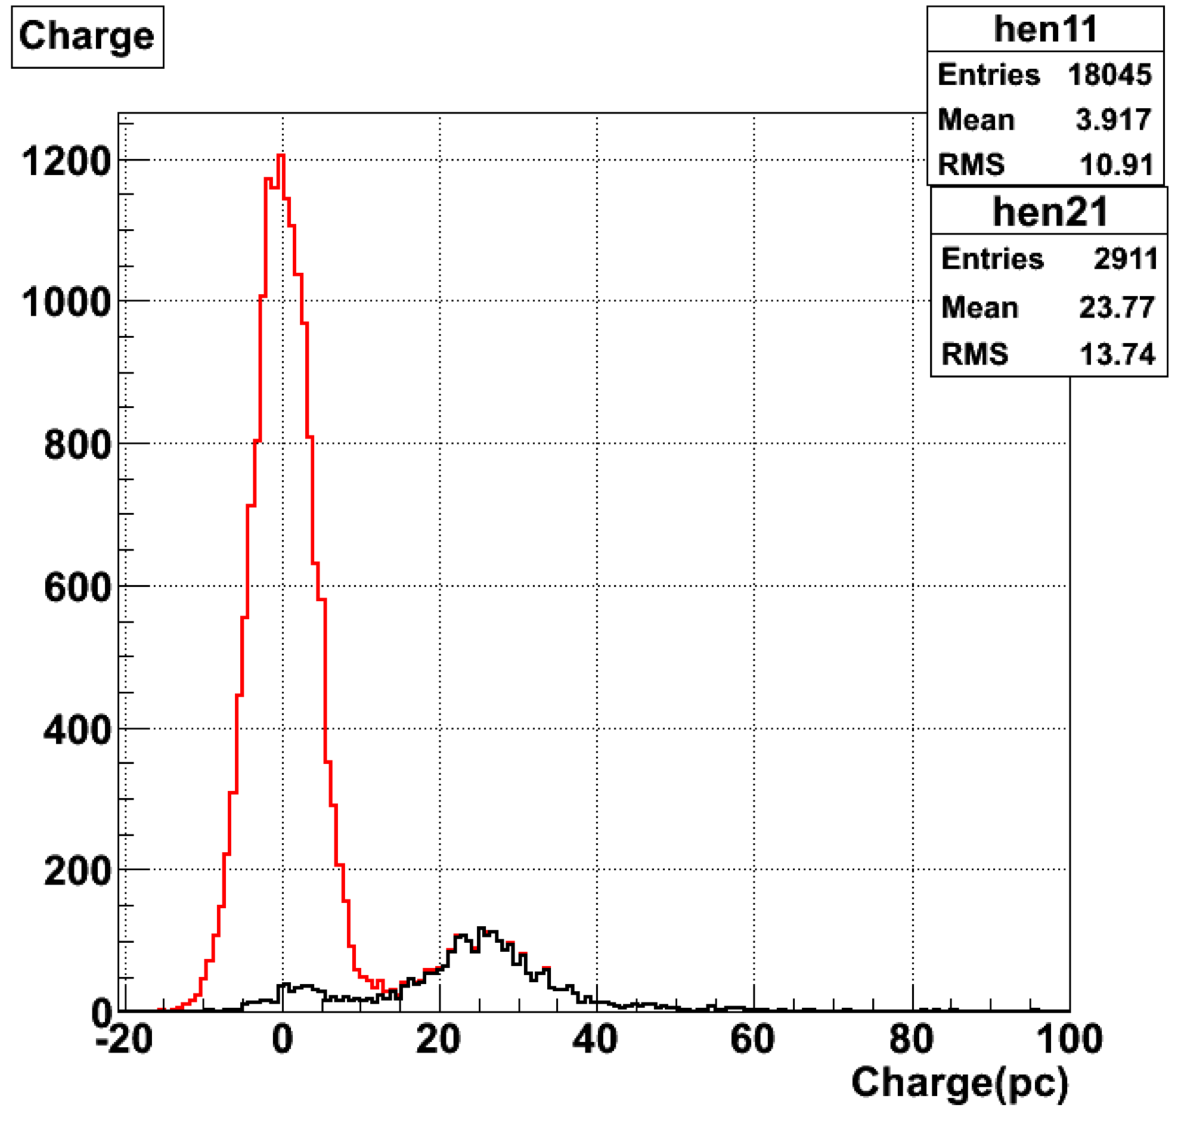
\includegraphics[scale=0.37]{ecal/MIP_10x10_APD.png}
\caption{\small{Charge distribution from readout of the HPS calorimeter crystal with Hamamatsu S8664-55 (left) and S8664-1010 
(right) APDs, and the new low noise amplifier board. The red line histogram corresponds to the charge distribution for all triggers 
comming from the scintillators positioned above and below the crystal. The black line shows the distribution for hits in the crystal 
within $100$ ns of the trigger signal. }}\label{fig:mip10x10}
\end{figure*}

\end{enumerate}


\subsection{Muon system {\it Keith, Yuri, Stepan, Larry}}

\label{sec:muon}


Searching for the A$^\prime$ in its di-muon decay mode has the advantage of having greatly reduced electromagnetic backgrounds for triggering.  The only physics background will arise from photoproduction of $\pi^+$ and $\pi^-$ pairs in the target, which aren�t fully absorbed in the ECal or absorber. The muon detector will be about 1 meter long and will consist of layers of scintillator hodoscopes sandwiched between iron absorbers. The number of layers and the thickness of absorbers is defined by the $\pi/\mu$ rejection factor. Detector was optimized using the GEANT-3 model of ECal, continued with layers of iron and scintillators. Muons in the momentum range from $1$ GeV to $4$ GeV has been studied, see \cite{HPS_PROP} for details.

In Figure \ref{fig:pmrej}, the rejection factor for charged pions is presented. As can be seen from the figure, for particles from $1$ GeV to $4$ GeV, the optimal thickness of the iron absorber for pion rejection is $\sim 75$ cm (after ECal, a $16$ cm of lead-tungstate). In the efficiency calculation for low energy particles ($< 1.7$ GeV) detection in in all four layers of scintillator hodoscopes were not considered. Depending on the momentum, particles were not traced behind the third, fourth or fifth absorber.  

\begin{figure*}[!ht]
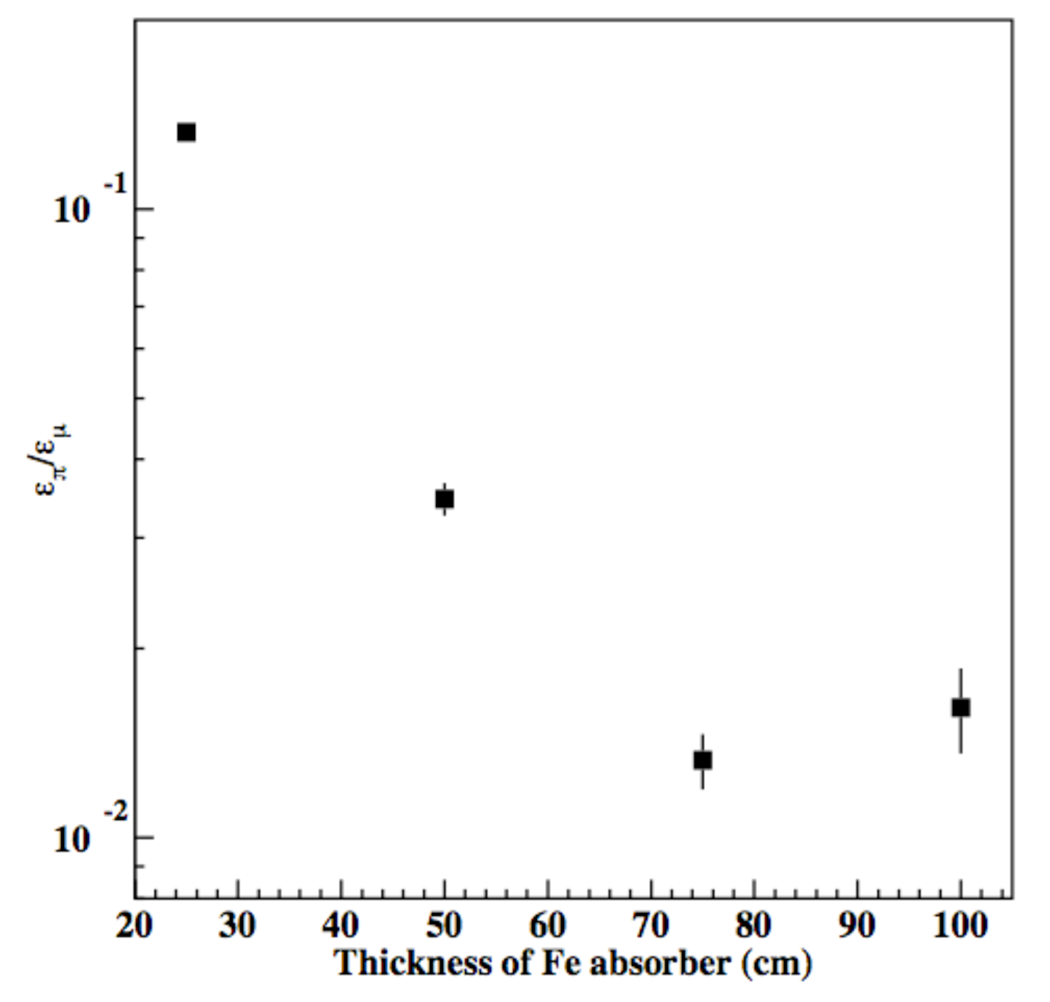
\includegraphics[scale=0.8]{muon/pmrej.pdf}
\caption{\small{Pion-muon rejection factor as a function of the iron absorber thickness.}}\label{fig:pmrej}
\end{figure*}


\subsubsection{Detector concept}

Based on simulations, a muon detector composed of a four iron absorbers (total length of $30+15+15+15=75$ cm) and four double-layer scintillator planes, positioned after each absorber layer is proposed. The muon detector will be mounted behind the ECal, see Figure 4.5.2.1. The pion rejection ($\pi/\mu$) of the proposed system as a function of particle momentum is shown in Figure \ref{fig:pmrejp}. For the determination of particle detection efficiencies, only signals in the first three layers of the hodoscope were used for momenta $< 1.7$ GeV/c. In the full momentum range from $1$ to $4$ GeV/c, $\pi/\mu$ varies from $10^{-2}$ to $2\times 10^{-2}$ and therefore the pion pair suppression factor of the system will be $< 4\times10^{-4}$. Similar to the Ecal, the muon detector will consist of two halves, one above and one below the beam. The vertical gap between the first hodoscope layers of the two halves is about 3 cm. The cross section of each half of the first hodoscope is $63\times 39$ cm$^2$. Each half of the last hodoscope layer is $74\times 46$ cm$^2$.  

\begin{figure*}[!ht]
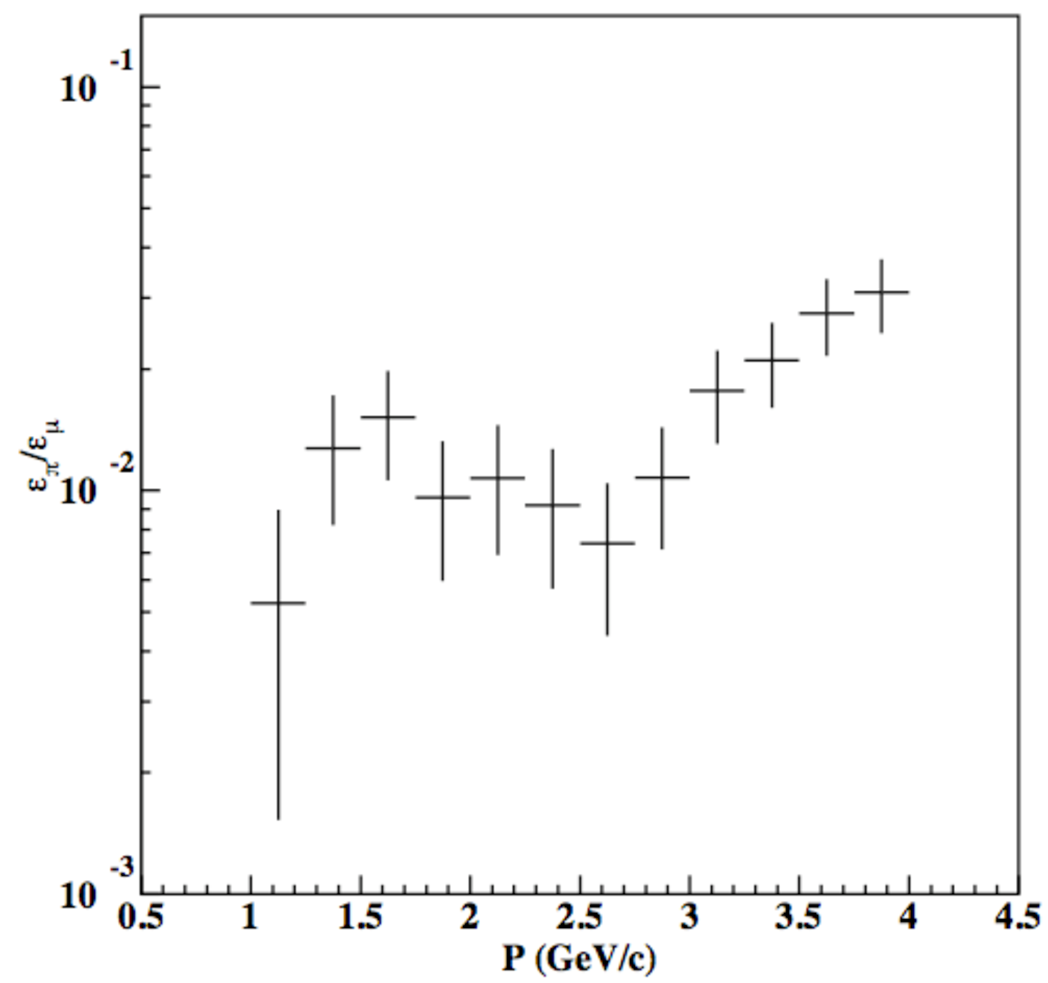
\includegraphics[scale=0.8]{muon/pmrej4.pdf}
\caption{\small{Pion-muon rejection factor as a function of the iron absorber thickness.}}\label{fig:pmrejp}
\end{figure*}

The simplest, most economical solution for the hodoscopes is to use layers of extruded scintillator strips with embedded wave-shifting fiber readout. The scintillator strips will be oriented horizontally. The light will be detected from both ends of the strip using multi-anode photomultipliers. With 5 cm vertical segmentation, a total of 144 readout channels are needed (9x16 channels multi-anode PMTs).  Signals from each channel will be sent to a TDC and to a FADC. The FADC information will be used to construct the muon trigger. The TDC information together with information from FADC will be used in offline analysis to measure the hit position along the strip. 

\clearpage

\section{Simulation Tools}
\label{app:sim}

The simulation tools play a critical role in simulating the background
environment, optimizing the detector setup, and developing the trigger 
and reconstruction strategies. We use GEANT4 and EGS5 to simulate 
electromagnetic interactions. There is generally good agreement 
between these two codes. In particular, no inconsistencies have been 
found on secondary particle yields or energy spectra. However, we have found 
significant disagreements on the angular distributions in the multiple
scattering, bremsstrahlung and pair production processes.  

%\vspace{1cm}
%\noindent
%{\bf Multiple Scattering}
\subsection*{Multiple Scattering Simulation}

EGS5 simulates the electron elastic scattering using the Moli\`{e}re theory 
\cite{moliere} as formulated by Bethe. \cite{bethe}
It is based on a small angle approximation
($\theta \ll$ 1 radian), and the angular distribution approaches asymptotically
to Gaussian at small angles, and to Rutherford's Coulomb scattering function at 
large angles given by, 
\begin{equation}
F(\theta) \sim  { \frac{1} {\left(1-cos\theta + {\frac{\chi^2} {2}}\right)^2}}.
\label{eq:rutherford}
\end{equation}

Instead of using the complex and time consuming Moli\`{e}re's formula,
GEANT4 uses two functions explicitly, Gaussian at small angles and the
Rutherford function Eq.~\ref{eq:rutherford} at large angles with a requirement that these two
functions and their first derivatives are joined continuously. 
GEANT4, however, uses a different power
in the denominator in Eq.~\ref{eq:rutherford} which is close to 2 but not exactly equal to 2 and is 
dependent on the target material and thickness.

Several comparisons have been made in the angular distribution $F(\theta)$ in the
differential cross section $d\sigma=F(\theta)d(cos\theta) d\phi$ for 2.2 GeV electron
scattering from 0.125\% $X_0$ Tungsten target. 
The EGS5 simulation is compared with Moli\`{e}re's analytical formula 
in Figure \ref{appendix:1}(a), demonstrating a good agreement between EGS5 and
the Moli\`{e}re theory.
While the Moli\`{e}re theory is based on a small angle approximation,
the multiple scattering theory developed by Gaudsmit and Saunderson is valid 
for any angle by means of an expansion in Legendre polynomials. \cite{gs}
The validity of the small angle approximation is checked by comparing the 
Moli\`{e}re integral with 
the Goudsmit-Saunderson theory as shown in Figure \ref{appendix:1}(b),
demonstrating that the Moli\`{e}re theory is accurate in the angular region
of the HPS detector. 

\begin{figure*}[ht]
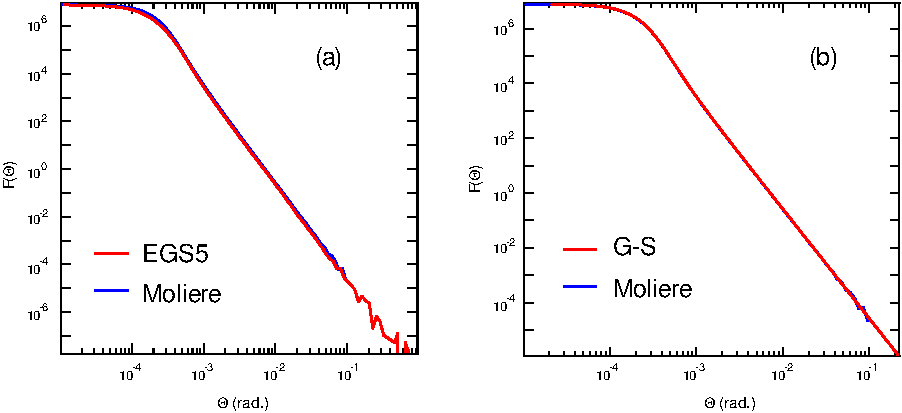
\includegraphics[height=3 in]{appendix/appendix_1-eps-converted-to.pdf}
\caption{\small{ (a) Moli\`{e}re vs. EGS5 \hspace{1 cm} (b) Moli\`{e}re vs. Goudsmit-Saunderson}}
\label{appendix:1}
\end{figure*}

Figure \ref{appendix:2} shows the angular distribution comparison between the GEANT4 
simulation and the Moli\`{e}re integral. 
GEANT4 is in good agreement with the Moli\`{e}re integral up to about 1 mrad, then it 
deviates at larger angles, predicting roughly twice the cross section at 15 mrad, 
where the HPS tracker sensor edge is located.

D. Attwood et al. measured 170 MeV muon angular distributions and compared with 
GEANT4 simulations and the Moli\`{e}re theory. \cite{attwood} They concluded that GEANT4 
simulation over-estimated the scattering tail by about a factor of two, and the data were consistent
with the Moli\`{e}re theory. G. Shen et al.~ \cite{shen} and B. Gottschalk et al.~ \cite{gottschalk}
also showed that the Moli\`{e}re theory was consistent with the measurements on a wide variety of
target materials.

\begin{figure}[ht]
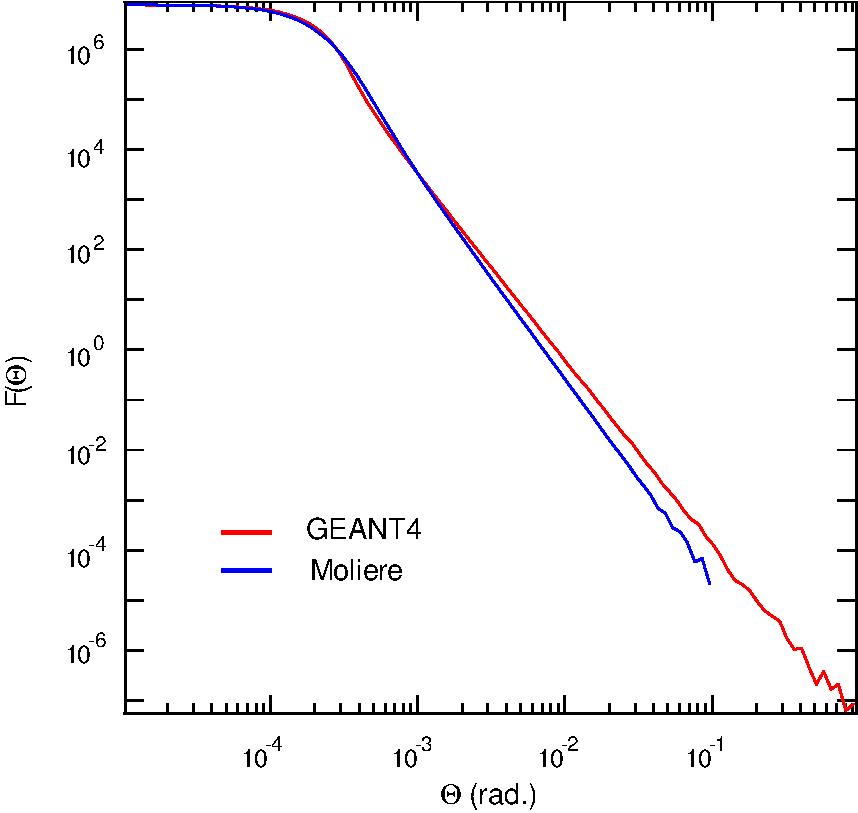
\includegraphics[height= 3 in]{appendix/appendix_2-eps-converted-to.pdf}
\caption{\small{ Moli\`{e}re vs. GEANT4 }}
\label{appendix:2}
\end{figure}

%\vspace{1cm}
%\noindent
%{\bf Angular distributions in the bremsstrahlung and pair production processes}
\subsection*{Angular Distributions}

While GEANT4 and EGS5 are in good agreement in the production rates and the secondary particle
energy spectra, there are significant differences in the angular distribution in the secondary
particles. In EGS5, the angular distributions are sampled from the following differential
cross section for the bremsstrahlung process, \cite{koch}

$$d\sigma(k,\theta_\gamma) = {\frac{4Z^2r_0^2} {137}} {\frac{dk} {k}} ydy\left\{{\frac{16y^2E} 
{(y^2+1)^4E_0}}
 -{\frac{(E_0+E)^2} {(y^2+1)^2E_0^2}}+\left\{{\frac{E_0^2+E^2} {(y^2+1)^2E_0^2}} -
 {\frac{4y^2E} {(y^2+1)^4E_0}}\right\} lnM(y) \right\}, $$

\noindent
where $k$ is photon energy, $\theta_\gamma$ is photon polar angle, $E_0$ and $E$ are initial and final 
electron energy, and

$$y=E_0\theta_\gamma; {\frac{1} {M(y)}} = \left({\frac{k} {2E_0E}}\right)^2 + \left({\frac{Z^{1/3}} {111(y^2+1)}}\right)^2, $$

\noindent
and for the pair production process, \cite{motz}

$${\frac{d\sigma} {dE_\pm d\Omega_\pm}} = {\frac{2\alpha Z^2r_0^2} {\pi}} {\frac{E_\pm^2} {k^3}}
\left\{-{\frac{(E_+-E_-)^2} {(u^2+1)^2}}-{\frac{16u^2E_+E_-} {(u^2+1)^4}} + \left\{ {\frac{E_+^2+E_-^2} 
{(u^2+1)^2}} + {\frac{4u^2E_+E_-} {(u^2+1)^4}} \right\} lnM(u)\right\},$$

\noindent
where $k$ photon energy, $E_\pm$ $e^{\pm}$ energy, $\theta_\pm$ $e^{\pm}$ polar angle, and

$$u=E_\pm\theta_\pm; {\frac{1} {M(u)}} = \left({\frac{k} {2E_+E_-}}\right)^2+\left({\frac{Z^{1/3}} {111(u^2+1)}}\right)^2.$$

\noindent
GEANT4 uses an approximate function to simulate the angular distributions in the 
bremsstrahlung and pair production processes given by

$$ f(u) = C [ue^{-au} + d u e^{-3au}], $$

\noindent
with $u=E_0\theta_\gamma$ for incident electron energy $E_0$ and the polar angle 
$\theta_\gamma$ of the bremsstrahlung photon, and $u=E_{\pm}\theta_{\pm}$ for the pair 
energy $E_\pm$ and polar angle $\theta_\pm$ in the pair production. Since the production angle
is typically $1/\gamma$, GEANT4's approximations are acceptable
for most of the high energy detector simulations. However, GEANT4
simulations are inconsistent with the data in the following two cases in the HPS Test Run:
\begin{itemize}
\item The bremsstrahlung photon angular distribution is too narrow, 
resulting in too few scatters in the collimator.
\item The prediction on the pair angular distribution is too narrow, resulting in 
too few Ecal trigger rates.
\end{itemize}

%\vspace{1cm}
%\noindent
%{\bf Conclusions}
\subsection*{Simulation Tools Setup in HPS}

Because of the inaccuracies in GEANT4 described above the electromagnetic interactions in the target are simulated 
by EGS5, and all the particles that come out of the target are passed on to the HPS detector 
simulation system based on GEANT4.


%\section{Production and Decay of the $A^\prime$}
\label{app:ProdAndDecay}

\def \ap {A^\prime}
\def \map {m_{A^\prime}}
\def \thap {\theta_{A^\prime}}


$\ap$ particles are generated in electron collisions on a fixed target by a process analogous to ordinary photon bremsstrahlung, see Figure \ref{fig:apdiagram}.  This can be reliably estimated in the Weizs\"acker-Williams approximation (see [1-4]).  When the incoming electron has energy $E_0$, the differential cross-section to produce an $\ap$ of mass $m_{\ap}$ with energy $E_{\ap}\equiv x E_0$ is 
\begin{equation}
\frac{d\sigma}{dxd\cos{\theta_{\ap}}}\approx \frac{8Z^2\alpha^3\epsilon^2 E_0^2 x}{U^2}\tilde{\chi}\times\left[\left(1-x+\frac{x^2}{2}\right)-\frac{x(1-x)m_{\ap}^2E_0^2x\theta_{\ap}^2}{U^2}\right]
\end{equation}
where Z is the atomic number of the target atoms, $\alpha = 1/137$,  is the angle in the lab frame between the emitted A' and the incoming electron, 
\begin{equation}
U(x,\theta_{\ap})=E_0^2x\theta_{\ap}^2+m_{\ap}^2\frac{1-x}{x}+m_e^2x
\label{eq:u}
\end{equation}
is the virtuality of the intermediate electron in initial-state bremsstrahlung, and  is the Weizs\"acker-Williams effective photon flux, with an overall factor of  removed.  The form of  and its dependence on the $\ap$ mass, beam energy, and target nucleus are discussed in \cite{Kim:1973he}.  For HPS with $E_0$ = 6.6 GeV, we find $\tilde{\chi}\sim 7 (4, 1)$ for $m_{\ap}$ = 100 (200, 500) MeV/$c^2$.
The above results are valid for 
\begin{equation}
m_e\ll m_{\ap}\ll E_0  , ~~ x\theta_{\ap}^2\ll 1.
\end{equation}
For $m_e\ll m_{\ap}$, the angular integration gives
\begin{equation}
\frac{d\sigma}{dx}\approx \frac{8Z^2\alpha^3\epsilon^2 x}{m_{\ap}^2}\left(1+\frac{x^2}{3(1-x)}\right)\tilde{\chi} .
\end{equation}

Assuming the $\ap$ decays into Standard Model particles rather than exotic, it's boosted lifetime is
\begin{equation}
l_0 \equiv \gamma c\tau \approx \frac{0.8 cm}{N_{eff}} \left(\frac{E_0}{10 GeV}\right)\left(\frac{10^{-4}}{\epsilon}\right)^2\left(\frac{100 MeV}{\map}\right)^2,
\end{equation}
where we have neglected phase-space corrections, and $N_{eff}$ counts the number of available decay channels.  If the $\ap$ couples only to electrons, then $N_{eff}=1$.  If the $\ap$ mixes kinetically with the photon, the $N_{eff}=1$ for $\map < 2m_\mu$ and $2+R(\map)$ for $\map \geq 2 m_\mu$, where \cite{eehadrons}
\begin{equation}
R  =\left. \frac{\sigma(e^+e^-\rarr hadrons)}{\sigma (e^+e^- \rarr \mu^+\mu^-)}\right|_{E=\map} . 
\end{equation} 
For the ranges of $\epsilon$ and $\map$ probed by this experiment, the mean decay length $l_0$ can be prompt or as large as tens of centimeters.  

The total number of $\ap$ produced when $N_e$ electrons scatter in a target of $T\ll 1 $ radiation lengths is
\begin{equation}
N\sim N_e\frac{N_0 X_0}{A}T\frac{Z^2\alpha^2\epsilon^2}{\map^2}\tilde{\chi}\sim N_e C T \frac{\epsilon m_e^2}{\map^2},
\end{equation}
where $X_0$ is the radiation length of the target in g/cm$^2$, $N_0 \approx 6\times 10^{23} mole^{-1}$ is Avogadro's number, and $A$ is the target atomic mass in g/mole.  The numerical factor $C\approx 5$ is logarithmically dependent on the choice of nucleus (at least in the range of masses where the form-factor is only slowly varying) and on $\map$, because, roughly, $X_0 \propto \frac{A}{Z^2}$ (see \cite{Kim:1973he, Essig:2010xa,Bjorken:2009mm}).  For a Coulomb of incident
electrons, the total number of $\ap$s produced is given by
\begin{equation}
N\sim 10^5 \left(\frac{N_e}{1 C}\right)\tilde{\chi}\left(\frac{T}{0.1}\right)\left(\frac{\epsilon}{10^{-4}}\right)^2\left(\frac{100 MeV}{\map}\right)^2.
\end{equation}



% \section{Test Run SVT Performance}
% \label{app:svt}
% \subsection*{SVT Calibration}

% 
%
%   svt_calibrations.tex
%       author: Omar Moreno <omoreno1@ucsc.edu>
%               Per Hansson <phansson@slac.stanford.edu>
%
%

In order to prepare the SVT for real physics data-taking, the SVT was 
calibrated. This involved the extraction of the mean baseline (pedestal),
baseline noise and gain for each of the 12,780 SVT channels. All measurements
were made with the APV25 readout chips configured to their nominal operating
points \cite{Jones:1069892} and all sensors biased to 180 V. The APV25s were
operated in ``mulit-peak'' mode with six samples being readout per trigger.
This, in turn, allowed for the extraction of the $t_0$ and amplitude of the 
signals being read out.

Figure~\ref{fig:pedestal_noise} shows an intensity plot of the pedestals 
along with the readout noise as a function of channel number for a single
hybrid.  The noise was computed by taking the RMS of the gaussian distributed
\begin{figure}[h]
    \begin{center}
    	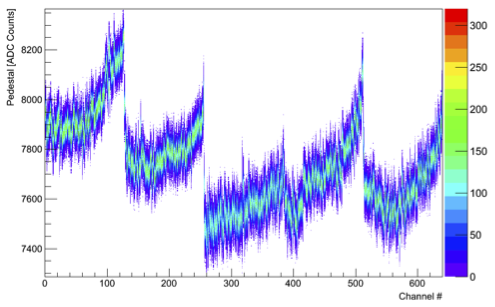
\includegraphics[width=0.45\textwidth]{test2012/svtperformance/baseline}
    	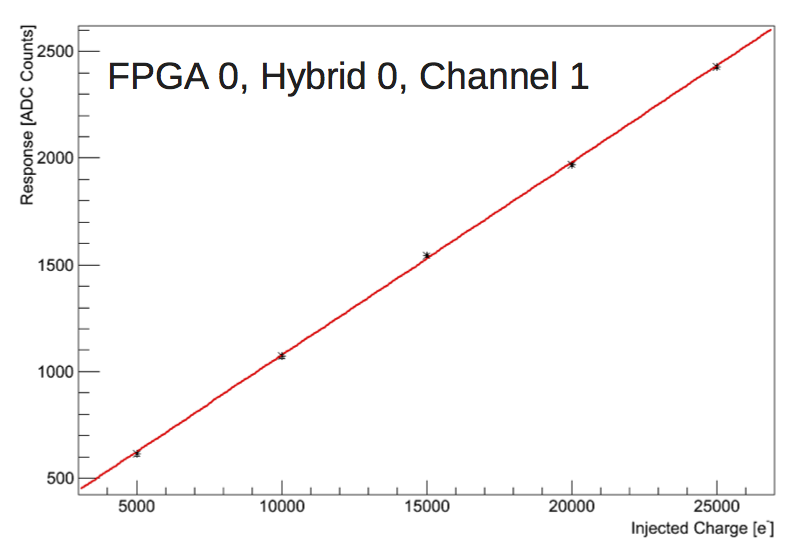
\includegraphics[width=0.45\textwidth]{test2012/svtperformance/gain}
        \caption{Something ... }
%    	\caption{\small{The baseline across a hybrid (left) and the measured response as a function of 
%	                    input charge (right). The overall shifts in the baseline are calibrated out where distinct edges 
%	                    are associated with the five APV25 chips on the hybrid. The gain shows good linearity up to 
%	                    about three $mip$s.} {\color{red}Should we show noise instead of baseline?}}
	\label{fig:pedestal_noise}
    \end{center}
\end{figure}
pedestals for each of the channels and was observed to be consistently within 
[Find number] ADC counts ( electrons).  One observed feature are the large
noise values for the channels lying near the chip edges.  This has also been 
reported by the CMS collaboration and the cause is still under investigation.

%  Need to rewrite this ...
Another important aspect for the characterization of the SVT is the response and the associated 
gain. Using the APV25 internal calibration circuit a known fixed charge was injected into all 
channels of the which allows for an accurate determination of the response and its 
scaling with input charge, shown in Fig.~\ref{fig:baseline_and_gain}. The gain uniformity was 
within the expected range across chips and modules and show good linearity of charge 
depositions up to about 3 $mip$s. 

All reconstructed hits in an event were used to form clusters of energy 
depositions using a nearest neighbor algorithm. Fig.~\ref{fig:cluster_pulse}
shows the mean pulse shape of each of the hits associated with a track as a 
function of time.  
\begin{figure}[h]
	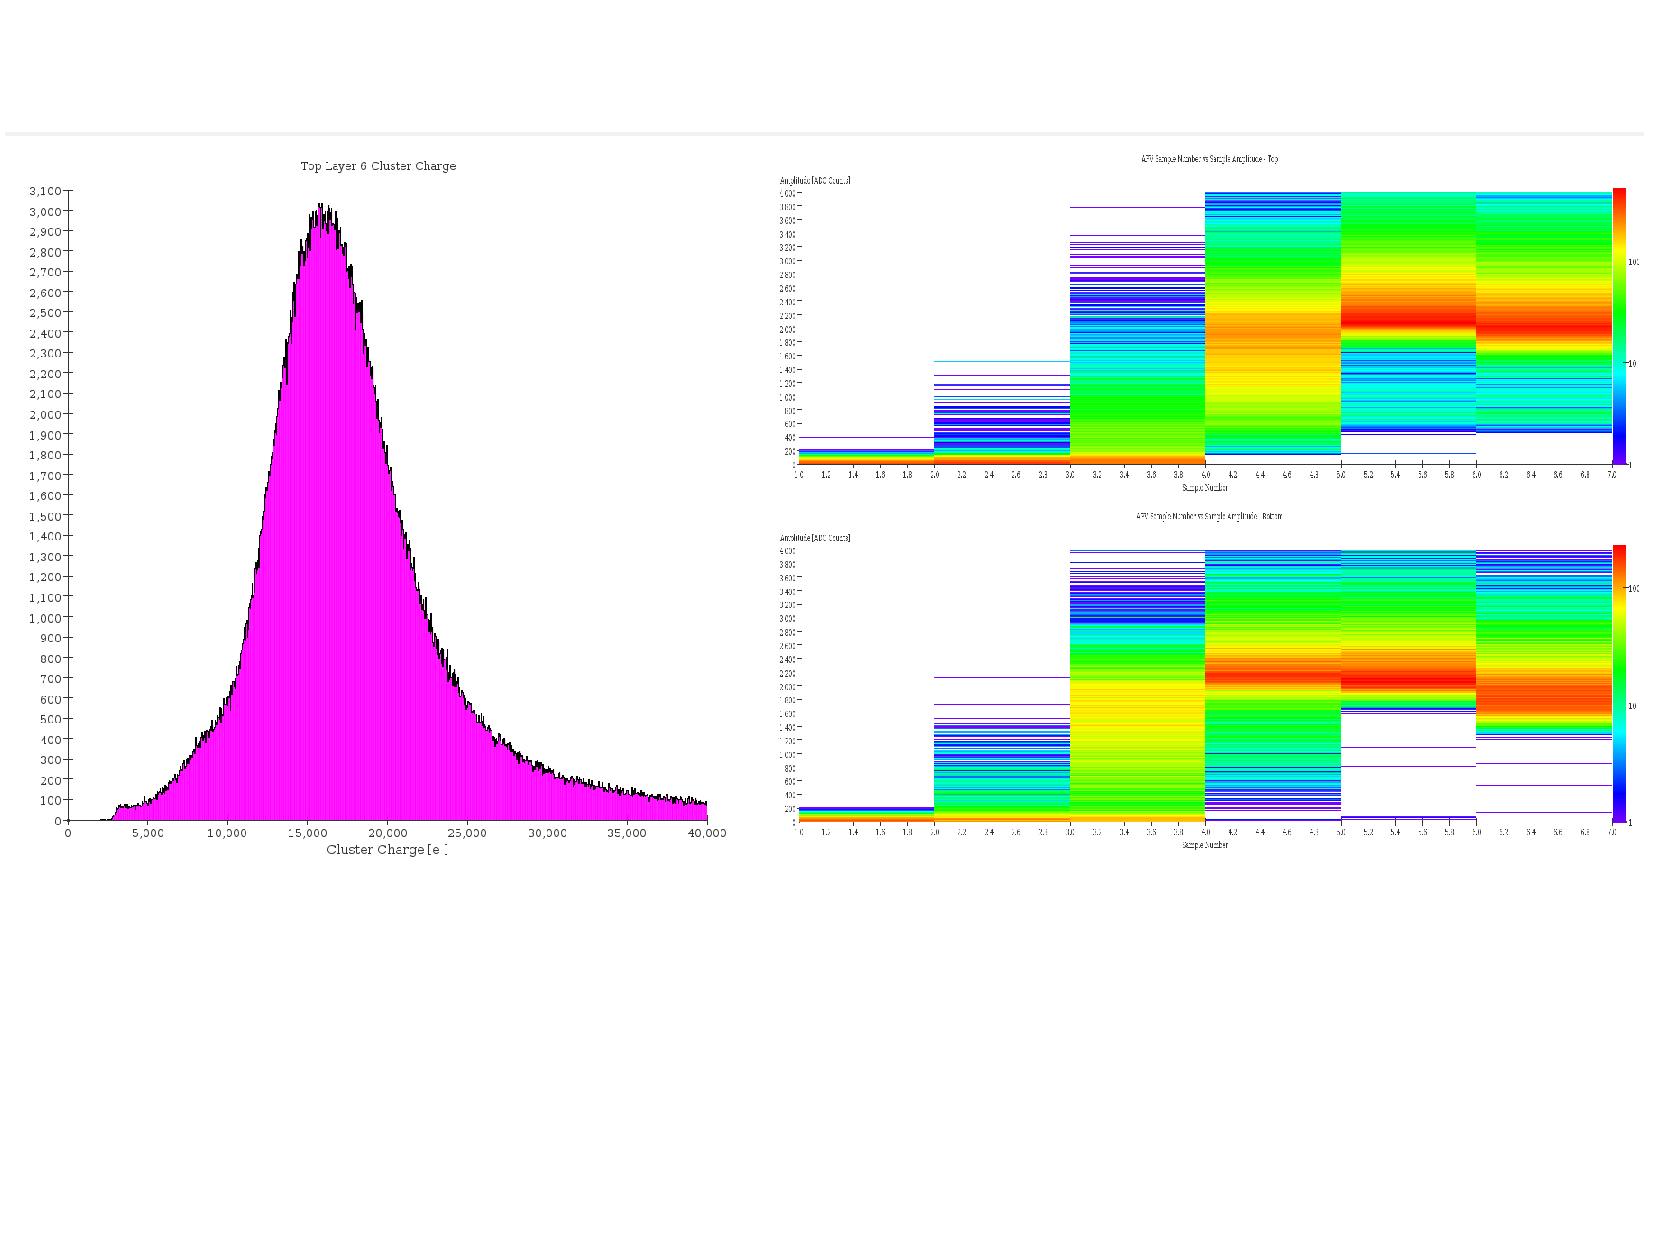
\includegraphics[width=\textwidth]{test2012/svtperformance/pulseshape_and_landau}
    \caption{Something else ...}
%	\caption{\small{The distribution of cluster amplitudes (left) showing the characteristic Landau 
%	shape and the pulse shape from the six samples readout (right) {\color{red} Remove one of the pulse shapes}. }}
	\label{fig:pulseshape}
\end{figure}
% Should this be included? If so, it needs to be rewritten a little better
The figure also demostrates that  the trigger system, described below, is well 
timed in with the tracker. 
Fig.~\ref{fig:cluster_pulse} shows the MIP response to be [Find value] electrons.
Taking the MIP response, the signal to noise ratio was calculated to be 
approximately 25.5 which is well matched to the expected behavior.

\bibliography{svt_calib}
 


% \subsection*{SVT Hit Time Resolution}
% As discussed in Sec.~\ref{sec:svt}, the APV25 multi-peak readout is crucial to the time stamping on hits
% in the SVT. This, in turn, allows the effective occupancies to be lowered for pattern recognition
% during electron running. 
% Six samples of the APV25 shaper output for each trigger are fitted to an ideal $CR-RC$ function to 
% extract the amplitude and hit time.  The $\chi^2$ distribution of these fits from test run data is as expected
% for four degrees of freedom.
% %\begin{figure}[]
% %	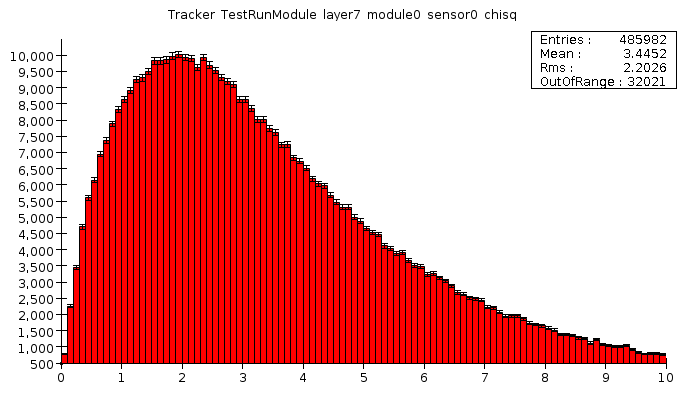
\includegraphics[width=0.6\textwidth]{test2012/svtperformance/apvfit_chisq}
% %	\caption{\small{Histogram of $\chi^2$ values for pulse fits for all channels on a representative sensor. The peak at 2 is consistent with 4 degrees of freedom (2 fit parameters), as expected. Pileup was not considered due to the very low hit rate in 
% %the SVT in this photon beam test. } }
% %	\label{fig:apvfit}
% %\end{figure}
% After clustering hits on a sensor, the hit time for each cluster is computed as the 
% amplitude-weighted average of the channel hit times. Since we have no measurement of the ``true'' hit time, we study the overall SVT hit 
% timing performance using the average of all cluster times in a track as the ``track time,'' and take the
%  residual of the cluster time relative to that. The observed track time, shown in Fig.~\ref{fig:tracktime}, has the expected amount of trigger jitter due to the readout clock and trigger system jitter. After correcting for offsets for each sensor (time-of-flight, clock phase) the RMS 
%  of the final residual distribution is roughly 2.4~ns for each sensor. 
% Because the track time is calculated using the individual hit times, the hit time is positively correlated 
% with the track time; thus the RMS of the residual is slightly smaller than the true time resolution.
% The standard deviation of this residual for $n$-hit tracks where all hits have the same time resolution 
% is reduced by a factor of $\sqrt{(n-1)/n}$; since most of our tracks have 8 clusters, the true time 
% resolution is 2.6 ns. 
% %\begin{figure}[ht]
% %	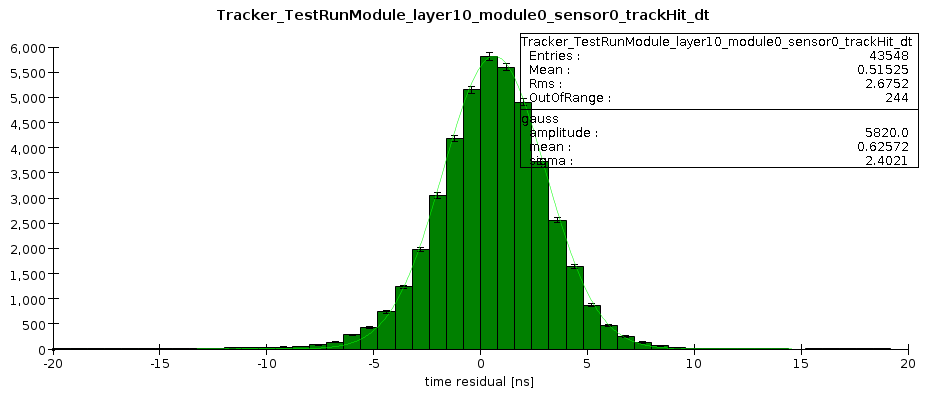
\includegraphics[width=\textwidth]{test2012/svtperformance/timeres}
% %	\caption{\small{Histogram and Gaussian fit of residual of cluster times for a representative sensor, relative to the track time. Because the cluster times and track time have positive covariance, the true time resolution is slightly larger than the standard deviation shown here.} }
% %	\label{fig:timeres}
% %\end{figure}
% %\begin{figure}[ht]
% %	\includegraphics[width=\textwidth]{test2012/svtperformance/hit_dt}
% %	\caption{\small{} }
% %	\label{fig:hit_dt}
% %\end{figure}
% This is somewhat worse than the $\approx 2$ ns resolution expected 
% %(see Fig.~\ref{fig:timeres}) 
% in 
% Sec.~\ref{sec:performance}, but we believe this discrepancy is due to our fit function. Our pulse 
% shape fit assumes an ideal CR-RC pulse shape; since the actual pulse shape has a slower rise time, 
% there is a systematic pull on the hit time when a hit comes immediately before the APV clock time. 
% This is visible in Figure \ref{fig:timeres_2D} as a shift in the residual at certain values of track time.
% \begin{figure}[ht]
% 	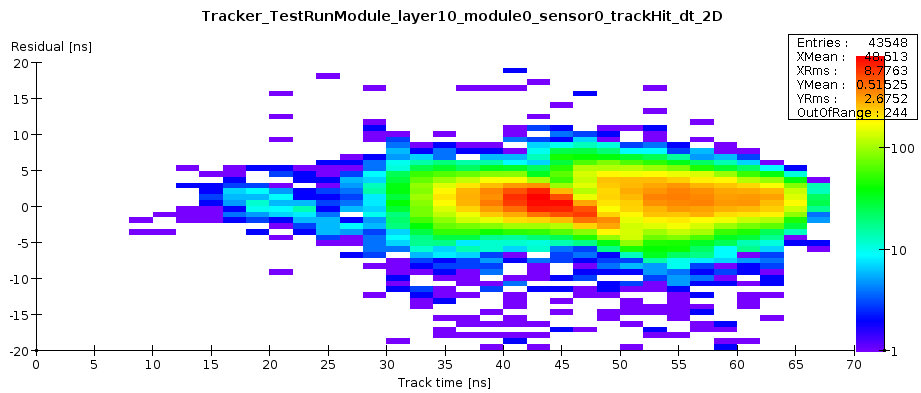
\includegraphics[width=0.7\textwidth]{test2012/svtperformance/timeres_2D}
% 	\caption{\small{Plot of the time residual for a representative sensor vs. the track time. 
% 		The kinks in the horizontal band are caused by the fitter; without them the time resolution (measured by taking the projection of this histogram) would be better.} }
% 	\label{fig:timeres_2D}
% \end{figure}
% Work is in progress to use the actual pulse shape in time reconstruction; this should improve time resolution to that expected from previous studies. 
% Reducing the APV25 pulse shaping time will also improve time resolution.
% In short, these results show that we can achieve time resolution adequate for pileup rejection during electron running.
% %\vspace{1cm}{\bf Tracking algorithms [Matt/Omar]}


% \subsection*{SVT Track Reconstruction}
% 
%
%   trk_performance.tex
%       author: Omar Moreno <omoreno1@ucsc.edu>
%      created: December 4, 2012
%
 
A charged particle traversing the sensitive volume of the SVT is expected to
deposit enough charge to produce hits which, in turn, are used to form 
clusters. Clusters which are in adjacent Si planes are then combined to form
2-dimensional ``stereo hits'' which are used by the tracking algorithm to 
form tracks.  The determination of the probability that a stereo hit is 
formed, or hit efficiency, provides insight as to the performance of each of 
the SVT layers.

In order to obtained the hit efficiencies, tracks were fit using only 4 of 
SVT layers. The resulting track was then extrapolated to the layer omitted
\begin{figure}[h]
    \begin{center}
        % TODO: Need to update the plot so that Layer 2 on the bottom doesn't 
        % look terrible. It's probably easiest to just remove the point altogether.
    	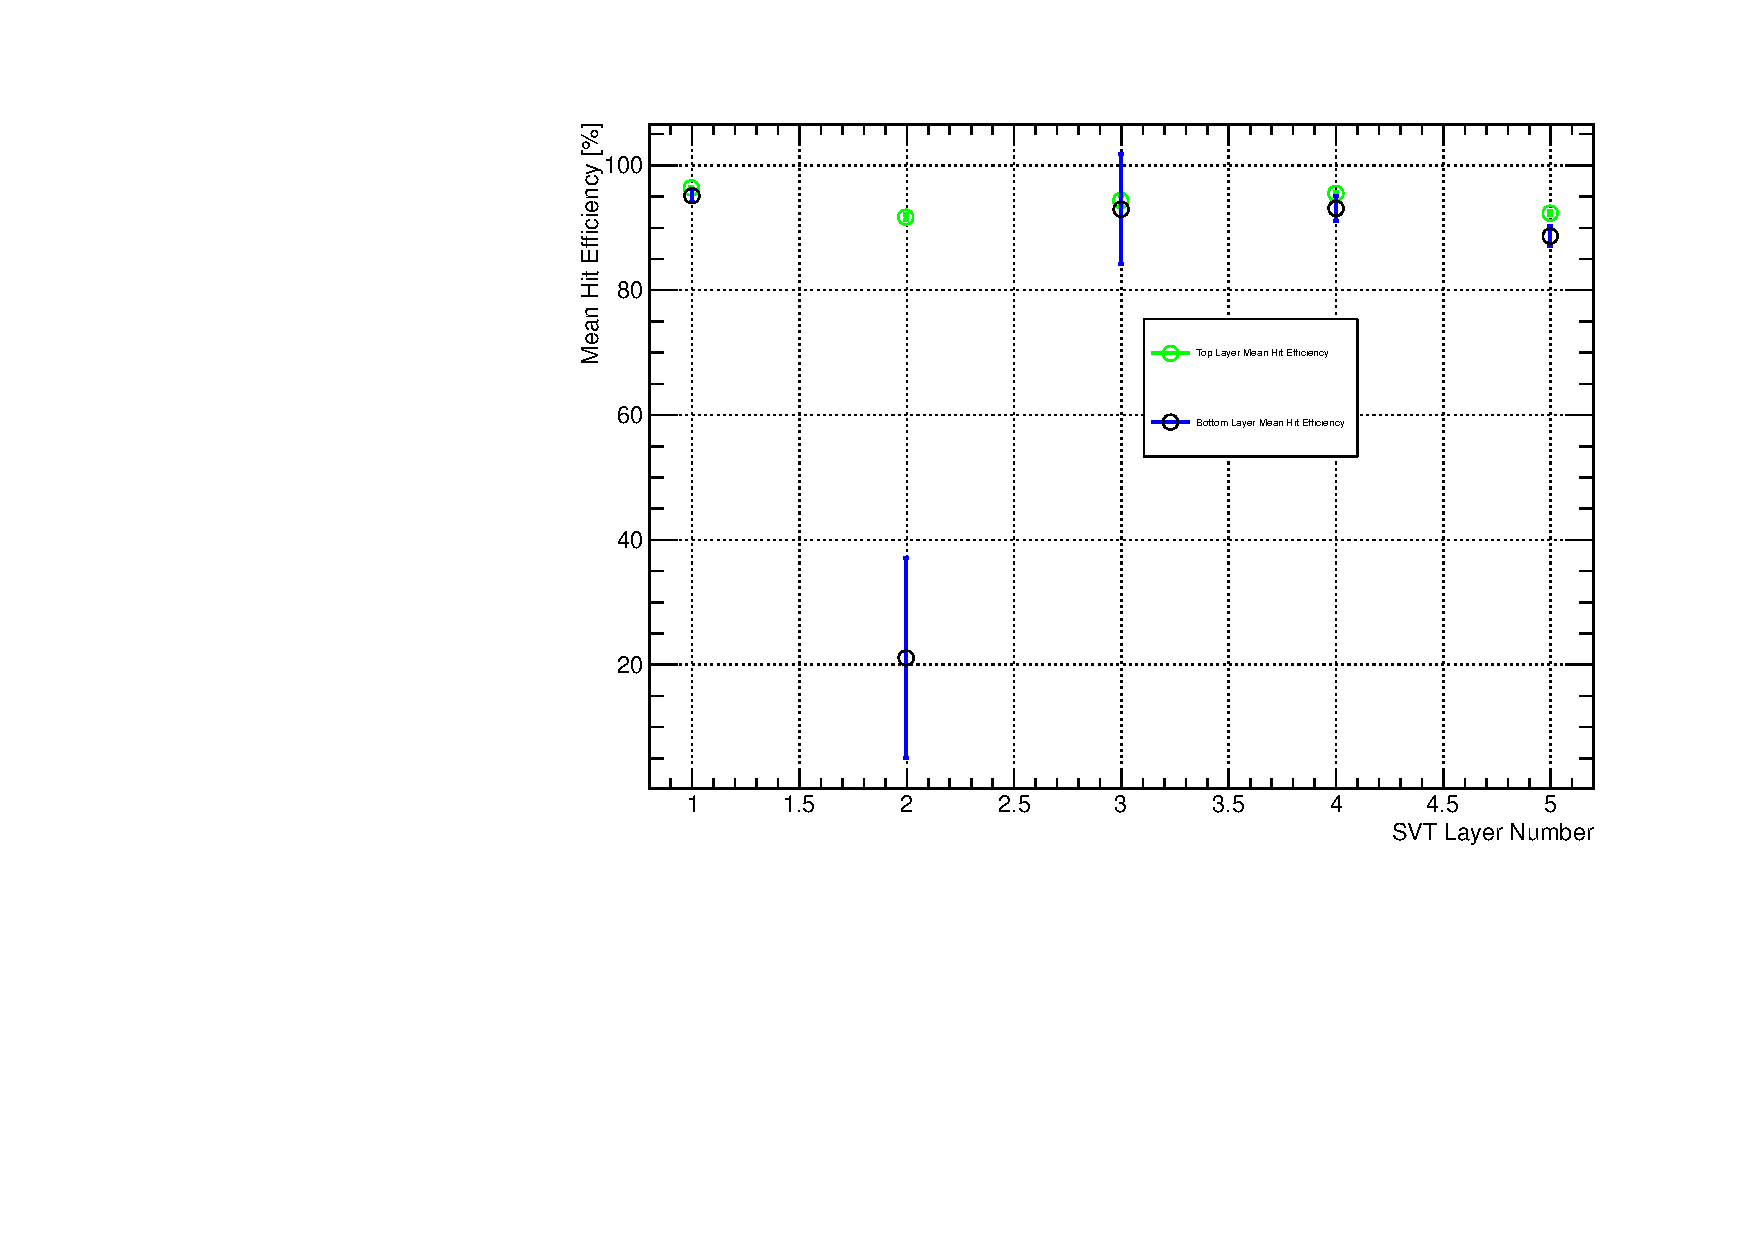
\includegraphics[width=0.49\textwidth]{test2012/svtperformance/trk_performance/mean_hit_efficiency_vs_layer.pdf}
    	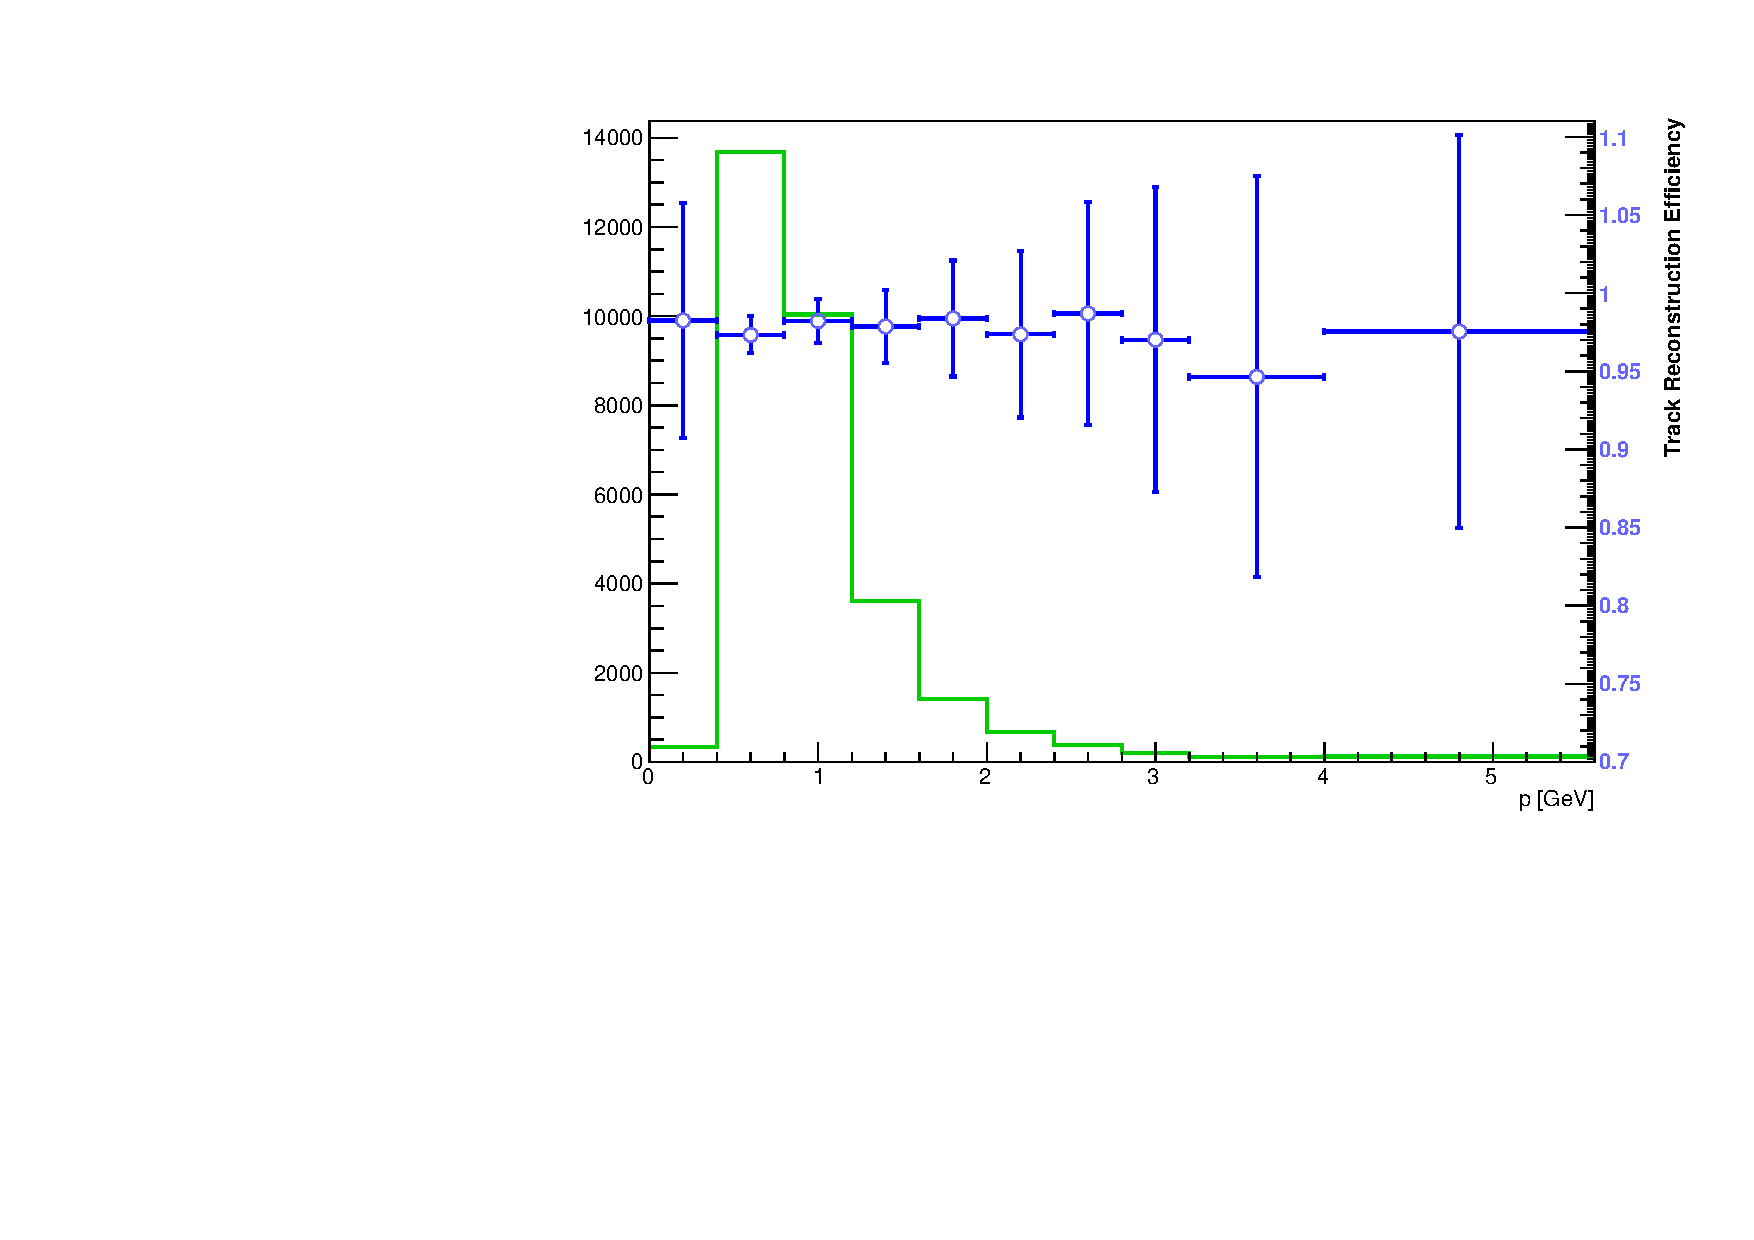
\includegraphics[width=0.49\textwidth]{test2012/svtperformance/trk_performance/track_reco_efficiency.pdf}
        \caption{
                    The plot on the left shows the average hit efficiency
                    from all dedicated photon runs as a function of layer
                    number.  Excluding known bad layers, the hit efficiency
                    is greater than 90\%. The track reconstruction efficiency
                    as a function of momentum (blue) along with the 
                    distribution of momenta for all tracks (green) is shown
                    on the right.
                } 
	\label{fig:hit_track_efficiency}
    \end{center}
\end{figure}
from the fit. If the track was found to lie within the sensitive volume
of the layer, a search for a stereo hit within the layer acceptance was 
conducted.  The hit efficiency was then determined as
\[
    \varepsilon_{\mbox{hit efficiency}} = \frac{\mbox{Tracks with hit on missing layer}}
                                            {\mbox{Tracks within layer acceptance}} \times 100 \%.
\]
The hit efficiencies per layer were calculated using all dedicated runs. As 
can be seen from Figure~\ref{fig:hit_track_efficiency}, the average hit efficiency
per layer, excluding all known bad Si sensors, was found to be greater than
90\%.
% The single hit efficiencies need to be updated to reflect changes that were 
% made to the tracking code

As mentioned above, the standard pattern recognition algorithm is designed to 
find tracks using the reconstructed stereo hits.  A set of tracking strategies
outline which layers should be used by the track finding algorithm along
with their role (seeding, extend, confirm), and the $\chi^2$ cut imposed 
on the fit. Any kinematic constraints are also specified within the strategy.
A detailed account of the tracking algorithm can be found  here~\ref{}.

In order to determine the efficiency of the track finding algorithm, a Monte
Carlo sample containing pair produced electrons from photons incident on 
a 1.6\% $X_0$ gold target was used.  The energy of the pair produced electrons
ranged from .5 GeV to 5.5 GeV. An electron falling within the detector 
acceptance was considered findable by the tracking algorithm if it 
traversed through at least 4 of the SVT layers. The track reconstruction
efficiency was then determined as
\[
    \varepsilon_{\mbox{track reco efficiency}} = \frac{\mbox{Tracks found}}
                                            {\mbox{Tracks found to be findable}} \times 100 \%.
\]
The resulting efficiency to find an electron which passes through the detector
acceptance is show on Figure~\ref{fig:hit_track_efficiency}. The average track
reconstruction efficiency was found to be \% with the bulk of the inefficiency
coming from the $\chi^2$ cut imposed on the fit to the six samples during
the clustering stage.

All events which contained pairs of oppositely charged tracks were fit to a
common vertex using a simple vertexing algorithm which searches for the distance
of closest approach between the two tracks.  The reconstructed vertex position
along the beam axis for both data and Monte Carlo is shown on 
Figure~\ref{fig:vz_position}.
\begin{figure}[h]
    \begin{center}
    	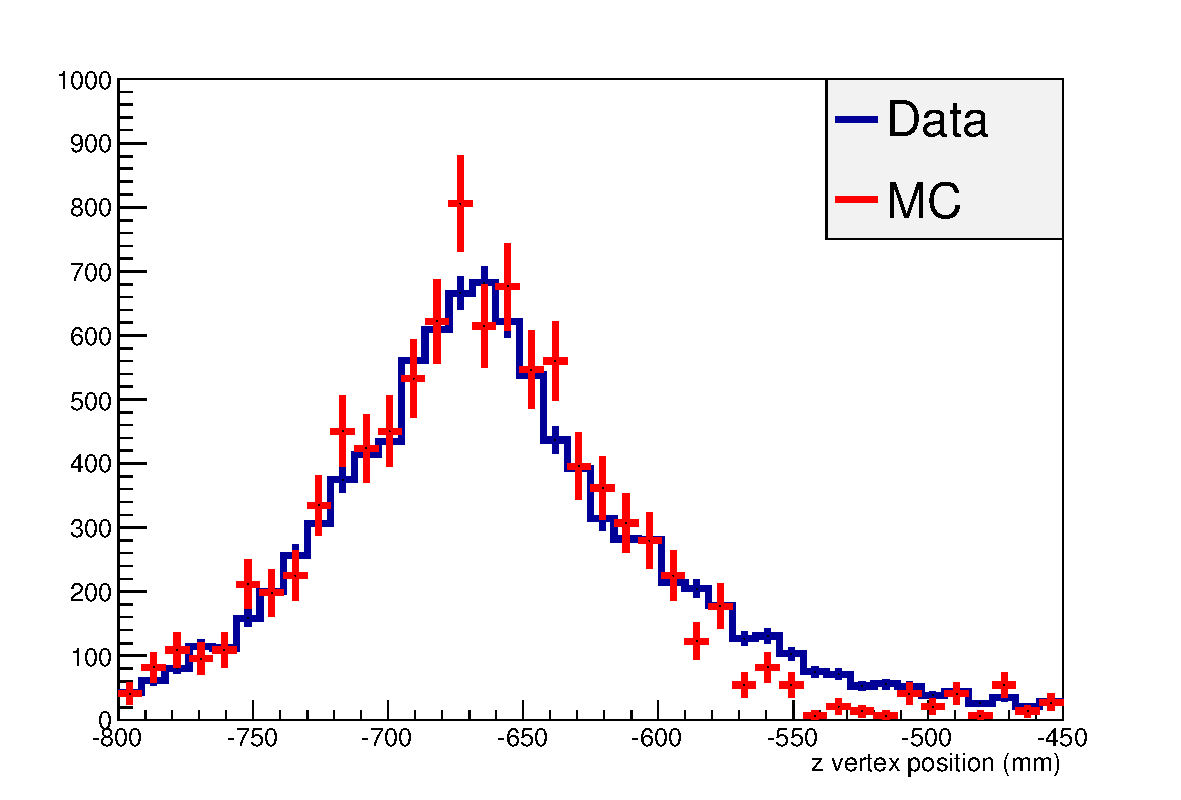
\includegraphics[width=0.60\textwidth]{test2012/svtperformance/trk_performance/zvertex.pdf}
        \caption{  
                    The reconstructed vertex position along the beam axis for
                    both data (blue) and Monte Carlo (red).
                } 
	\label{fig:vz_position}
    \end{center}
\end{figure}
Because of the geometric setup of the SVT, observation of pairs produced by
the incident photon required both electrons to multiple scatter a significant 
amount within the target.  This results in a broadening of the Gaussian 
distributed reconstructed vertex position as seen in the Figure. 



% \subsection*{SVT Test Run DAQ Performance}
% 
%
%   svt_daq.tex
%       author: Omar Moreno <omoreno1@ucsc.edu>
%               Santa Cruz Institute for Particle Physics
%               University of California, Santa Cruz
%      created: November 13, 2012
%

The expected data rates and event sizes for each of the dedicated photon runs
were estimated using a full simulation of the SVT DAQ and compared to observed
values. As discussed in Section~\ref{sec:testrun_daq}, the digitized samples
from three hybrids were received by a single DPM.  The DPM then required that
at least three of the six samples exceeded a threshold of two times the noise
level for that channel.  An additional ``pile-up'' cut requiring that 
(sample 2 $>$ sample 1) or (sample 3 $>$ sample 2) was also applied. This was
meant to eliminate hits arising from the falling edge of previous hits expected
to occur when running at the highest occupancies.
%Signals from the photon run were unaffected by such a cut. 

All samples were placed into their own container along with the 
channel number, hybrid identifier, chip address and DPM identifier. An 
additional layer of encapsulation or bank was used to store all samples 
emerging from a single DPM along with the DPM identifier, the event number
an error bit and hybrid temperatures. A diagram of the container along with
the sizes of each of the elements is shown on Figure~\ref{fig:data_format}.
\begin{figure}[h]
    \begin{center}
    	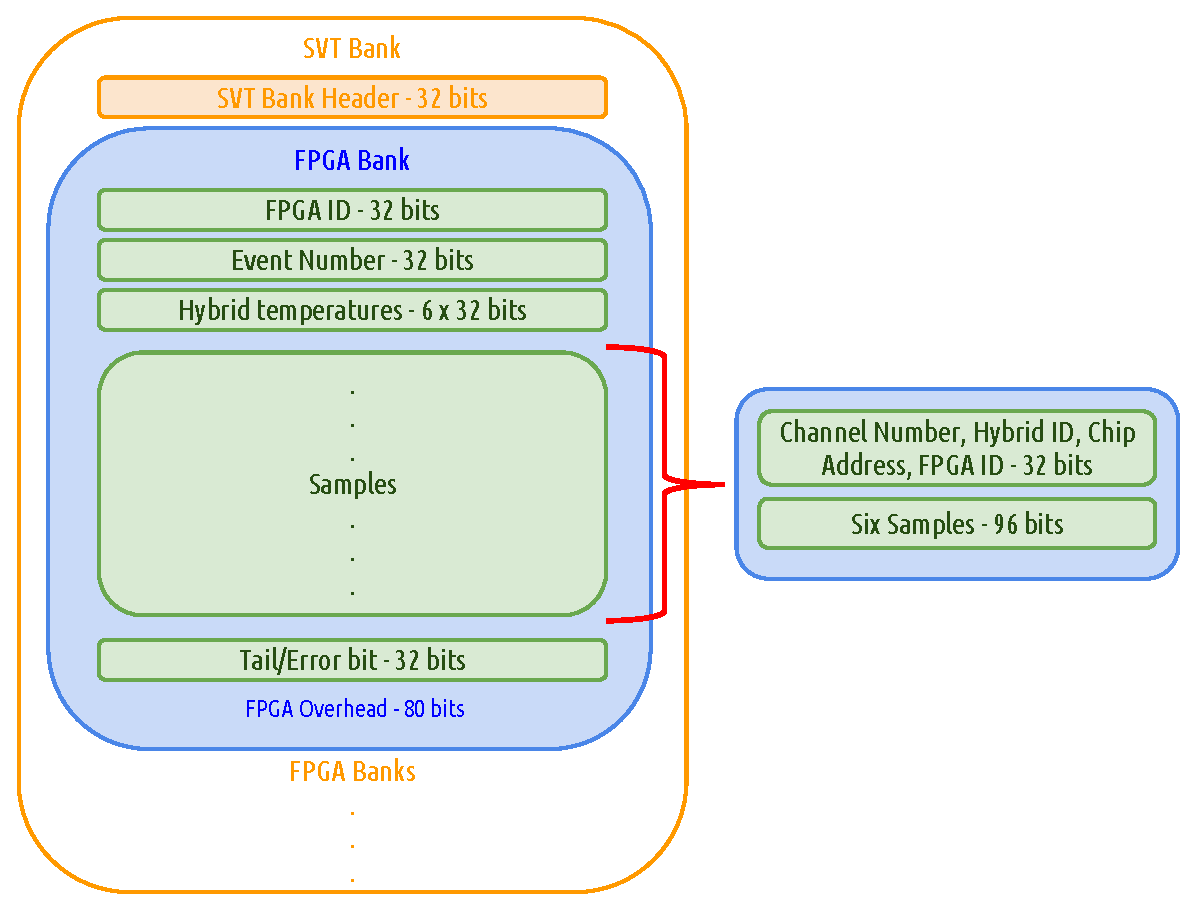
\includegraphics[width=0.60\textwidth]{test2012/svtperformance/daq/svt_data_format.pdf}
        \caption{
                    SVT data format. Samples readout from three hybrids are 
                    processed by a single FPGA and are placed within a single
                    container or FPGA bank.  An additional layer of 
                    encapsulation is used to store all of the FPGA banks.
                 } 
	\label{fig:data_format}
    \end{center}
\end{figure}
Overall, the container overhead will contribute a total of 326 bytes to an event
with an additional 16 bytes per hit.

The occupancy expected for each of the converter thicknesses along with the 
corresponding event size and data rate are shown on Table~\ref{table:sim_rates}.
\begin{table}[h]
    \scalebox{0.9}{
    \begin{tabular}{ c | c | c | c }
    \hline
    %  Are the trigger rates going to be listed anywhere else? Otherwise, they should be listed here.
    Converter Thickness (\%$X_0$) & Sim Occupancy (\%)  & Sim Event Size (kB) &   Sim Data Rate (Mb/s) \\      
    \hline 
    1.6                           & .438                & 1.22                &   2.07                 \\
    0.45                          & .293                & .93                 &   .53                  \\
    0.18                          & .118                & .56                 &   .24                  \\ 
    \end{tabular} } 
    \caption{Occupancy, event size and resulting data rate expected for each of the three 
             converter thicknesses used in the test run.}
    \label{table:sim_rates}
\end{table}
The occupancies shown include a contribution of .02\% (3 hits) due to noise and  
data rates are estimated using the trigger rates observed during each
of the dedicated photon runs. As expected i.e. thicker targets correspond to higher 
occupancies. 

Table~\ref{table:observed_rates} list the observed occupancy, event sizes and 
\begin{table}[h]
    \scalebox{0.9}{ 
        \begin{tabular}{ c | c | c | c }
            \hline
            Converter Thickness (\%$X_0$)   & Obs. Occupancy (\%) & Obs. Event Size (kB) & Obs. Data Rate (Mb/s) \\
            \hline
            1.6                             & 1.03                & 2.43                 & 4.12                  \\
            0.45                            & 1.22                & 2.82                 & 1.61                  \\
            0.18                            & 1.23                & 2.84                 & 1.21                  \\
        \end{tabular}
    }
    \caption{Occupancy, event size and resulting data rate observed for each of the three 
             converter thicknesses used in the test run.}
    \label{table:observed_rates}
\end{table}    
rates for each of the targets.  The data rates observed during the test run were
much higher than expected.  This can be attributed to a known
noisy sensor and a few noisy chips which appeared during certain runs.  The causes
of both these issues are now well understood and will be resolved for future running.

A better comparison between simulated and observed data rates can be obtained
by masking out all known noisy channels found during the commissioning of the 
SVT.  The resulting data rates are listed on Table~\ref{table:masked_rates}. 
\begin{table}[h]
    \scalebox{0.8}{ 
        \begin{tabular}{ c | c | c | c }
            \hline
            Converter Thickness (\%$X_0$)   & Obs. (Sim) Occupancy (\%) & Obs. (Sim) Event Size (kB) & Obs. (Sim) Data Rate (Mb/s) \\
            \hline
            1.6                             &  ()               &  ()                &   ()                \\
            0.45                            &  ()               &  ()                &   ()                \\
            0.18                            &  ()               &  ()                &   ()                \\
        \end{tabular}
    }
    \caption{Comparison of occupancy, event size and resulting data rate for each of the three 
             converter thicknesses used in the test run after all bad channels are masked.}
    \label{table:masked_rates}
\end{table}    
\textcolor{red}{Combine all tables into a single plot.}


\section{Test Run ECal Calibration}
\label{sec:ecal_calib}

%The noise and pedestal of the readout chain are calibrated by running the ECal readout in a mode where the preamplifier output is sampled every 4~ns in a time window of 100 samples: by looking at a part of the window before the hit, we calibrate the readout channel.
The noise and pedestal of the readout chain are calibrated by sampling the preamplifer output out-of-time with the trigger.

We calibrate gain of the individual ECal channels using the SVT measurement of track momentum and comparison to Monte Carlo simulation. 
% The ratio of cluster energy to track momentum is calculated both for Monte Carlo simulation and test run data at each point in the ECal, and we find the value of gain for each channel that brings the two into agreement.
We disable all SVT and ECal channels in the simulation that were inoperable or noisy in the test run, so any efficiency or bias effects that affect the real data should be reflected in the simulation as well; then we use a formula to compute the ``weighted E/p'' for a crystal, representing the average E/p for clusters that include the crystal: $\frac{\sum_j w_{j,i}}{\sum_j\frac{P_j}{E_j}w_{j,i}}$, and iteratively adjust the gains until the weighted E/p is equal for test run data and simulation.

% The calibrated gains are corrected by the ratio between the weighted E/p values from Monte Carlo and real data.
% The E/p in Monte Carlo data is also affected by the gain because the trigger thresholds change, so both Monte Carlo and data reconstruction are rerun with each iteration of gain calibration.
% It takes up to 4 iterations for the gains to stabilize; the final values are shown in Figure \ref{fig:gains}.
\begin{figure}[ht]
	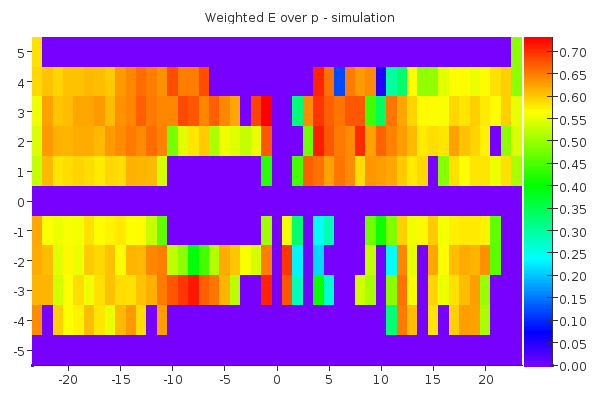
\includegraphics[width=0.45\textwidth]{test2012/ecalperformance/ecalgainplots_corr_sim}
	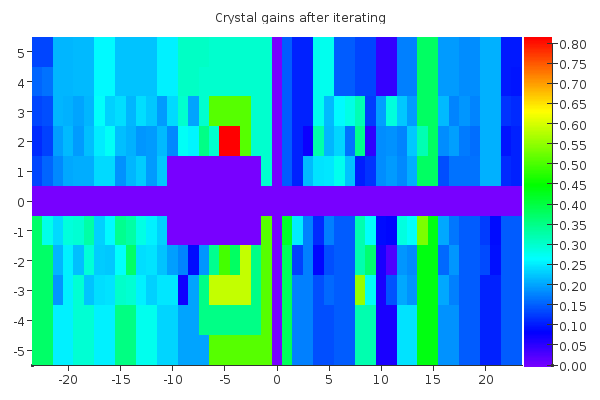
\includegraphics[width=0.45\textwidth]{test2012/ecalperformance/gains}
	\caption{\small{Weighted E/p from Monte Carlo simulation (left), calibrated values of gain in units of MeV per ADC count (right).}}
	\label{fig:gains}
\end{figure}

These gains can then be used to convert from ADC counts in a channel to the energy deposited into that ECal crystal.
The other information needed to find the energy of an incident particle is the sampling fraction---the ratio of energy read out from crystals to energy of an incident particle.
The conventional sampling fraction---the fraction of incident energy that is deposited in crystals---is approximately 0.9 for our ECal, and less at edges.
For our readout, there is additional energy lost because crystals under the readout threshold are not read out.
The weighted E/p used in calibration (see Figure \ref{fig:gains}) is an approximate measurement of sampling fraction, but the sampling fraction is energy-dependent because of the effect of readout threshold. 
A full computation of sampling fraction can be done using simulation.
